%\newcommand{\myFontSize}[0] {10pt}
%\newcommand{\mySpacing}[0] {1.1}
\newcommand{\myFontSize}[0] {10pt}
\newcommand{\mySpacing}[0] {1}

\newcommand{\thesisTitle}[0] {Evaluating Recommender Systems for Digital Library Datasets}
%Odporúčacie systémy založené na AI
\documentclass[\myFontSize,a4paper,oneside,hidelinks]{article} 

%\documentclass[\myFontSize,a4paper,twoside,openright,english,hidelinks]{book} 
%%%%%%%%%%%%%%%%%%%%%%%%%%%%%%%%%%%%%%%%%%%%%%%%%%%
\renewcommand{\familydefault}{\rmdefault}	% Serif Font by default

\usepackage[english, slovak]{babel}
\usepackage{graphicx}
%\usepackage{newtxtext}	% Times new Roman
\usepackage{float}
\usepackage{longtable}
\usepackage{enumitem}
\usepackage{setspace}
\usepackage{url} 
\usepackage{doi} 
\usepackage{cite}
\usepackage{comment} 
\usepackage[utf8]{inputenc}
\usepackage{enumitem}
\usepackage{titlesec}
\usepackage{multicol}
\usepackage{hyperref}
\usepackage[a4paper, top=3cm, bottom=3cm, left=2.5cm, right=2.5cm]{geometry}
\usepackage[parfill]{parskip}
\usepackage{glossaries}
\usepackage{array}
\usepackage{tikz}
\usepackage{pdfpages}
\usetikzlibrary{arrows.meta, positioning, calc}
\usepackage{listings}
\usepackage{lipsum}
\usepackage{xcolor}  % for custom colors
%%%%%%%%%%%%%%%%%%%%%%%%%%%%%%%%%%%%%%%%%%%%%%%%%%%




\definecolor{codegray}{gray}{0.95}
%\lstset{
%  backgroundcolor=\color{codegray},
%  basicstyle=\ttfamily\normalsize,
%  frame=single,
%  breaklines=true,
%  showstringspaces=false,
%  tabsize=2,
%  language=Python
%}

%%%%%%%%%%%%%%%%%%%%%%%%%%%%%%%%%%%%%%%%%%%%%%%%%%%

\setstretch{\mySpacing}
\setcounter{tocdepth}{3}

\makeglossaries

%%%%%%%%%%%%%%%%%%%%%%%%%%%%%%%%%%%%%%%%%%%%%%%%%%%
\begin{document} 
\selectlanguage{english}

\begin{center}
\thispagestyle{empty}
{\Large Slovak University of Technology in Bratislava}
\par\end{center}{\Large \par}

\begin{center}
{\Large Faculty of Informatics and Information Technologies} \\[1em]
{\Large FIIT-16768-121314}
\par\end{center}{\Large \par}

\smallskip{}

\vfill{}

\begin{center}
\textbf{\Large Ákos Lévárdy}
\par\end{center}{\Large \par}

\medskip{}

\begin{center}
\textbf{\Large \thesisTitle}
\par\end{center}{\Large \par}

\medskip{}

\begin{center}
{\Large Bachelor's thesis}
\par\end{center}{\Large \par}

\vfill{}

\Large{
Study programme: Informatics\\ 
Study field: Computer Science\\ 
Place: Institute of Informatics, Information Systems and Software Engineering\\ 
Supervisor: PaedDr. Pavol Baťalík\\\\
May 2025
%\today
}

%\maketitle
%\thispagestyle{empty}
%\vspace{4\baselineskip} 		% vertical space 
%\hspace{-2cm} 					% horizontal position
%\parbox{0.8\textwidth}{ 
%\raggedright 					% Left-align the text
%
%%%%%%%%%%%%%%%%%%%%%%%%%%%%%%%%%%%%%%%%%%%%%%%%%%%

\titleformat{\section}{\huge\bfseries}{\thesection}{1em}{}
\titleformat{\subsection}{\LARGE\bfseries}{\thesubsection}{1em}{}
\titleformat{\subsubsection}{\Large\bfseries}{\thesubsubsection}{1em}{}

%
%\tiny
%\scriptsize
%\footnotesize
%\small
%\normalsize
%\large
%\Large
%\LARGE
%\huge
%\Huge
%

\newpage{}
\thispagestyle{empty}
\mbox{}


\includepdf[pages=1]{zadanie.pdf}

\newpage{}
\thispagestyle{empty}
\mbox{}

\newpage{} 		% Čestné vyhlásenie
%\setcounter{page}{4}
\pagenumbering{gobble}
\vspace*{\fill}
\noindent \Large \textbf{Declaration of honour}\\
\noindent I declare on my honour that I wrote this thesis single-handed with usage of quoted literature and based on my knowledge and professional supervision of my supervisor PaedDr. Pavol Baťalík.\\\\

\begin{flushleft}
In Bratislava, 12.05.2025
\end{flushleft}

\begin{flushright}
\underline{\hspace{4cm}}\\\hfill
Ákos Lévárdy
\end{flushright}
\vspace*{\fill} 
\vspace{-8cm} 



\newpage 			% Poďakovanie
%\setcounter{page}{4}
\pagenumbering{gobble}
\vspace*{\fill} 
\noindent \Large \textbf{Acknowledgement}\\
\noindent First and foremost, I would like to thank my supervisor for their invaluable guidance and support throughout the duration of this project. I would also like to thank Ing. Jakub Dubec, whose assistance and feedback were greatly appreciated.
\vspace*{\fill} 
\vspace{-8cm} 




\newpage{} 
\thispagestyle{empty}
\section*{Annotation}
\begin{minipage}[t]{\columnwidth}%
Slovak University of Technology Bratislava\\
%
\textsc{\large FACULTY OF INFORMATICS AND INFORMATION TECHNOLOGIES}
%
\begin{tabbing}
Degree Course: \hspace{2.5em} \=Informatics\\\\
%
Author: \> Ákos Lévárdy\\	% \thesistitle
Bachelor's Thesis: \> \parbox[t]{0.6\textwidth}{Evaluating Recommender Systems for\\Digital Library Datasets}\\
Supervisor: \> PaedDr. Pavol Baťalík\\
2025, May
\end{tabbing}
%\today%
\end{minipage}
\bigskip{}

% 984 characters
This bachelor thesis focuses on analysing and evaluating recommender systems best suitable for digital library datasets. With the rise of digital content, such systems help users navigate large information spaces by generating personalized recommendations. In the introduction we show the importance and role of Recommender Systems (RS) in filtering and anticipating user preferences across various domains. We then present an overview of the key recommendation techniques, explaining their underlying mechanisms and common challenges. The project emphasizes Content-Based Filtering techniques, comparing text representational methods like BERT, FastText, LSA, and TF-IDF. 
Offline experiments were conducted to evaluate the system’s ability to generate Top-N book recommendations from the input data and the algorithms were compared based on evaluation metrics such as similarity, coverage, diversity or confidence. 
The main objective of this work aims to design and implement a system capable of benchmarking different recommendation algorithms designed for digital library datasets and to provide insights into their effectiveness and applicability in this domain.

%\newpage{}
%\thispagestyle{empty}
%\mbox{}

\newpage{}
\thispagestyle{empty}
\section*{Anotácia}
\begin{minipage}[t]{\columnwidth}%
Slovenská technická univerzita v Bratislave\\
%
\textsc{\large FAKULTA INFORMATIKY A INFORMAČNÝCH TECHNOLÓGIÍ}
%
\begin{tabbing}
Študijný program: \hspace{3em} \= Informatika\\\\
%
Autor: \> Ákos Lévárdy \\
Bakalárska práca: \>\parbox[t]{0.6\textwidth}{Vyhodnocovanie odporúčacích systémov pre datasety digitálnych knižníc}\\
Vedúci bakalárskej práce: \> PaedDr. Pavol Baťalík\\
Máj, 2025
\end{tabbing}
%\today%
\end{minipage}
\bigskip{}

% 1037 characters
Táto bakalárska práca sa zameriava na analýzu a hodnotenie odporúčacích systémov, ktoré sú najvhodnejšie pre datasety digitálnych knižníc. S rastom digitálneho obsahu tieto systémy pomáhajú používateľom orientovať sa v rozsiahlych informačných priestoroch generovaním personalizovaných odporúčaní. 
V úvode je predstavený význam a úloha odporúčacích systémov pri filtrovaní a predpovedaní používateľských preferencií v rôznych oblastiach. Práca následne poskytuje prehľad kľúčových odporúčacích techník, pričom vysvetľuje ich základné princípy a bežné problémy. Projekt kladie dôraz na techniky založené na obsahovom filtrovaní, pričom porovnáva rôzne prístupy na reprezentáciu textu, ako BERT, FastText, LSA alebo TF-IDF.
Boli vykonané offline experimenty na vyhodnotenie schopnosti systému generovať odporúčania Top-N kníh na základe vstupných dát. Algoritmy boli testované a porovnávané podľa hodnotiacich metrík ako napríklad podobnosť, pokrytie, diverzita alebo dôvera.
Hlavným cieľom tejto práce je navrhnúť a implementovať systém schopný porovnávať rôzne odporúčacie algoritmy určené pre digitálne knižničné dáta a poskytnúť prehľad o ich efektívnosti a použiteľnosti v danej oblasti.



%%%%%%%%%%%%%%%%%%%%%%%%%%%%%%%%%%%%%%%%%%%%%%%%%%%

\newpage{} 
\pagenumbering{roman}
\setcounter{page}{9}
\renewcommand{\contentsname}{Table of Contents}
\tableofcontents


%%%%%%%%%%%%%%%%%%%%%%%%%%%%%%%%%%%%%%%%%%%%%%%%%%%
%\newacronym{ai}{AI}{Artificial Intelligence}
%\newacronym{ml}{ML}{Machine Learning}

\newpage{}
\listoffigures
\listoftables
\printglossary[type=\acronymtype, title=List of Abbreviations]


\newpage{}
\thispagestyle{empty}
\mbox{}




%\section*{List of Abbreviations}


%%%%%%%%%%%%%%%%%%%%%%%%%%%%%%%%%%%%%%%%%%%%%%%%%%%
% \hspace{1.3em}

\clearpage{} 
\pagenumbering{arabic}
\setcounter{page}{1}

\section{Introduction}
%artificial \gls{ai}\\
%machine \gls{ml}\\

As Internet and Web technologies continue to evolve rapidly, the amount of information available online has expanded excessively across sections such as e-commerce, e-government or e-learning. To help users navigate this vast sea of content, Recommender Systems (RS) have become fundamental. These systems are not designed just for saving time for users, but they are enhancing the users experience when using the said system, by anticipating their needs and relevant items or topics to discover. They are very effective tools for filtering out the most appropriate information any user would like to find. The primary focus of these recommendations is to predict if a specific user will be interested in the distinct items.\\
%
“Item” is the general term used to refer to what the system recommends to users. A RS normally focuses on a specific type of item (e.g., movies, books or news) and accordingly its design, its graphical user interface, and the core recommendation technique used to generate the recommendations are all customized to provide useful and effective suggestions for that specific type of item. \cite{pub.1036183961}\\
%
The basic principle of recommendations is that significant dependencies exist between user- and item-centric activity. 
For example, a user who is interested in a historical documentary is more likely to be interested in another historical documentary or an educational program, rather than in an action movie. \cite{pub.1022525812}\\
%
Making decisions is not always easy. People are frequently presented with an overwhelming number of options when picking a product, a movie, or a destination to travel to, and each option comes with different levels of information and trustworthiness. \\
While there are many situations in which users know exactly what they are looking for and would like immediate answers, in other cases they are willing to explore and extend their knowledge \cite{Blanco201333}.\\
%
The main target of this project is to create a recommendation system that uses different algorithms in the topic of  book recommendations and evaluate these algorithms based on specified metrics.\\




%%%%%%%%%%%%%%%%%%%%%%%%%%%%%%%%%%%%%%%%%%%%%%%%%%%

\clearpage{}
\section{Understanding Recommendation Systems}

The main purpose of \textbf{Recommendation Systems} is to predict useful items, select some of them and after comparing them, the system recommends the most accurate ones.\\ 
These personalized recommendation systems are emerging as appropriate tools to aid and speed up the process of information seeking, considering the dramatic increase in big data \cite{Haruna2017}. They need to handle a large amount of textual data in order to accurately understand users’ reading preferences and generate corresponding recommendations \cite{Yan2024}. \\
%
%Because of this number of detail from all of the items, recommendation systems are becoming increasingly important. They help reduce options and offer better suggestions for the user so that they will have a personalized list to select their favourite. Fast and efficient access to relevant information is essential in any field of study. \\
%
Similarly, \textbf{Search Engines} are essential for navigating the vast amount of information available online. They make it possible for people to quickly look up solutions, learn new things, and browse the wide variety of resources on the internet. Search engine optimization is now necessary to guarantee that search engines deliver relevant results, quick search times, and a top-notch user experience given the explosive growth of online information.\\
A search engine is essentially a software that finds the information the user needs using keywords or phrases. It delivers results rapidly, even with millions of websites available online.
The importance of speed in online searches is highlighted by how even minor delays in retrieval can negatively affect users' perception of result quality \cite{pub.1171882357}.\\
%
While both Recommendation Systems (Information Filtering techniques) and Search Engines (Information Retrieval techniques) aim to help users navigate all this information, they do it differently. Personalized recommendation systems make suggestions based on past user behavior and preferences, whereas search engines use keyword-based searches to retrieve content from a selection of sources.\\
%
Information systems often deal with changing data over time. The term called Concept drift describes when sometimes the patterns or behaviors in the data change unexpectedly which affects how the system makes predictions \cite{Sun2024}.\\
The task to provide users with currently available options for products that fit their requirements and interests is very important in todays consumer society. These products are mostly supplied by inputs \cite{Philip2014} , sometimes even matching the users distinct tastes.\\
%
When someone is trying to find a movie to watch, it would be hard for them to start searching without any starting options. After all a blank page and no suggestions to choose from might even make the user decide not to pick anything. \\
%
%\newpage{}
Recommending items can be done in a variety of ways. Several types of recommendation systems exist, and their methods of operation differ. Below are different recommendation systems listed.

%These recommendation types can be divided into 3 main categories, which are Content-Based Filtering approaches (CB), Collaborative Filtering approaches (CF) and Hybrid approaches which are the combinations of the two. \\
%Other categories also include Knowledge-Based, Context-Aware, Popularity-Based, Demographic, Utility-Based and Deep Learning-Based Recommendation.\\\\
%

%{
%\begin{table}[h!]
%\centering
%\renewcommand{\arraystretch}{1.3} 
%{\Large
%\begin{tabular}{m{0.03\textwidth}|m{0.5\textwidth}}
%\hline
%\textbf{\# } & \textbf{Category} \\ \hline
%1. & Content-Based Filtering (CB) \\ \hline
%2. & Collaborative Filtering (CF) \\ \hline
%3. & Hybrid Approaches \\ \hline
%4. & Knowledge-Based \\ \hline
%5. & Context-Aware \\ \hline
%6. & Popularity-Based \\ \hline
%7. & Demographic \\ \hline
%8. & Utility-Based \\ \hline
%9. & Deep Learning-Based \\ \hline
%\end{tabular}
%}
%\caption{Types of Recommendation Systems}
%\label{table:recommendation-systems}
%\end{table}
%}


%
\textbf{Basic ideas of the recommendation techniques:}
\begin{itemize}[label=--]
\item \textbf{Content-Based Filtering} works in a way that it creates user profiles and suggests the individual items or products based on the users past choices with similar items. The items have various features and characteristics which connect them \cite{pub.1034486657}.
\item \textbf{Collaborative Filtering} relies more on preferences of other users and their behaviour. The point is that users who had similar interests before will have them again in the future for new items \cite{NILASHI2018507}.
\item \textbf{Knowledge-Graphs} use a network of data where items are linked through their features. Showing how items relate to one another and connecting them with more information and detail \cite{Imene2022488}.
\item \textbf{Context-Aware} recommendation systems are adding contextual factors to the rating process, where the recommended item is based on the users explicit ratings, the items implicitly inferred ratings and also the contextual variables  \cite{Haruna2017}. The variables for example when recommending a movie can be the location from where the user watches the movie, the time and the companion who the user watches the movie with.
\item \textbf{Popularity-Based} recommendations offer products that are popular or well-liked by a lot of users. They assume that these popular items are likely to be of interest to the majority of users, not considering their personal preferences.
\item \textbf{Demographic} recommendation systems are recommending items based on a demographic profile of the user. They categorize the users from their personal attributes and try to make user stereotypes \cite{Burke2002331}.
\item \textbf{Utility-Based} systems generate the recommendations by computing the utility of each item for the user. The utility of an item refers to how valuable it is to a user and is calculated using a utility function which combines different factors of the user's preferences \cite{Burke2002331}.
\item \textbf{Deep Learning-Based} are trying to find complex patterns in the users behaviour and the items features using deep learning algorithms and neural networks. These models can locate hidden links and can offer highly customized recommendations.
\item \textbf{Hybrid methods} try to combine the useful characteristics of both collaborative filtering and content-based filtering methods. They take into account both the users past preferences and the preferences of other people who might share the users taste \cite{melville:aaai02}.
\end{itemize}
%
%\newpage{}
\subsection{Role of Recommendation Systems}
The Recommendation System can have a range of roles to play. First it is important to distinguish on whose behalf the role is played, which can be either the service providers or the users side. For example, a recommendation system for music, implemented by a streaming service like Spotify wants to increase user engagement by recommending new playlists and songs, which leads to more subscriptions or advertisement revenue. While on the other hand the user wants to listen to personalized playlists and discover songs they might like.\\
There are more ways why a service provider would want to utilize such technology: \cite{pub.1036183961}
\begin{itemize}
\item Sell more items - to be able to sell additional items beyond those which are normally sold without recommendations. To increase the number of users that accept a recommendation and consume an item.
\item Sell more diverse items - not just to sell the most popular items, but also recommend items that might be hard to find. The popular items will probably be sold either way, on the other hand the service provider might want to sell every item.
\item Increase user satisfaction - improve the experience for the user with effective recommendations and combine it with a usable interface, so the user will be more satisfied with the system.
\item Increase user fidelity - make more personalized recommendations based on the users previous visits and interactions, by treating the user as a valuable customer.
\item Better understand what the user wants - to describe the user's preferences which are explicitly collected or predicted by the system. The service provider can even use this knowledge for other goals like improve inventory management or target specific promotions. \\
\end{itemize}
%
From the users point of view the recommendation system can help in implementing other core tasks which are normally associated with an RS. The popular tasks are the following: \cite{Ricci20221}

\begin{enumerate}[label=\textbf{\arabic*.}]
    \item Find some good items - Identify a selection of quality items.
    \item Find all good items - Locate all available items deemed good.
    \item Annotate items in context - Emphasize items based on the user's preferences and context.
    \item Recommend a sequence - Suggest an order for engaging with items.
    \item Recommend a bundle - Propose a set of complementary items together.
    \item Just browsing - Explore items without the intention of purchasing.
    \item Find credible recommender - Evaluate how effective the system is at making recommendations.
    \item Improve the active user's profile - Enhance the system's understanding of the user's preferences.
    \item Express self - Share opinions and provide ratings to assist the system.
    \item Help others - Evaluate items to guide others in finding what suits them.
    \item Influence others - Persuade other users to consider particular products.
\end{enumerate}


%\begin{table}[h!]
%\centering
%{
%\renewcommand{\arraystretch}{2}
%{\large
%\begin{tabular}{|m{0.03\textwidth}|m{0.3\textwidth}|m{0.6\textwidth}|}
%\hline
%\textbf{\#} & \textbf{Task} & \textbf{Description} \\ \hline
%1. & Find some good items & Identify a selection of quality items. \\ \hline
%2. & Find all good items & Locate all available items deemed good. \\ \hline
%3. & Annotate items in context & Emphasize items based on the user's preferences and context. \\ \hline
%4. & Recommend a sequence & Suggest an order for engaging with items. \\ \hline
%5. & Recommend a bundle & Propose a set of complementary items together. \\ \hline
%6. & Just browsing & Explore items without the intention of purchasing. \\ \hline
%7. & Find credible recommender & Evaluate how effective the system is at making recommendations. \\ \hline
%8. & Improve the active user's profile & Enhance the system's understanding of the user's preferences. \\ \hline
%9. & Express self & Share opinions and provide ratings to assist the system. \\ \hline
%10. & Help others & Evaluate items to guide others in finding what suits them. \\ \hline
%11. & Influence others & Persuade other users to consider particular products. \\ \hline
%\end{tabular}
%}
%}
%\caption{Recommendation System tasks}
%\label{table:rs-tasks}
%\end{table}

%%%%%%%%%%%%%%%%%%%%%%%%%%%%%%%%%%%%%%%%%%%%%
\clearpage

\subsection{Recommendation Techniques}
From a higher perspective recommendation techniques are generaly categorized into three approaches which are Collaborative Filtering, Content-Based Filtering and Hybrid Approaches. These methods differ in how they generate recommendations and offer unique advantages. The efficiency of a recommender system greatly depends on the type of algorithm used and the nature of the data source, which may be contextual, textual, visual etc. \cite{Roy2022}\\
In the following section the techniques Collaborative Filtering, Content-based Filtering, Knowledge Graphs and Hybrid Approaches are described in more detail.
%
\subsubsection{Collaborative Filtering}
One of the most popular methods used for personalized recommendations is collaborative filtering (CF). This method filters information from users, which means it compares users behaviour, interactions with items and data, item correlation and ratings from users. \\
It can perform in domains where there is not much content associated with items, or where the content is difficult for a computer to analyze - ideas, opinions etc.\cite{melville:aaai02}\\
Collaborative filtering can be divided into 2 methods which are "Memory-based" and "Model-Based" collaborative filtering. The first one relies on historical preferences, whereas the second method is based on machine learning models to predict the best options.\\\\
%
\textbf{Memory-based CF}\\
Collaborative filtering systems based on memory automate the common principle that similar users prefer similar items, and similar items are preferred by similar users \cite{Ning201537}. \\
This method can also be called Neighborhood-based and is further divided into 2 basic types, which are:
\begin{itemize}
\item User-Based Collaborative Filtering
	\begin{itemize}
	\item The main idea is that 2 completely distinct users who have an interest in a specific item and they rate this item similarly will probably be drawn to a new item the same way.
	\end{itemize}
\item Item-Based Collaborative Filtering
	\begin{itemize}
	\item Calculates similarity between items, rather than users. The user will probably like a new item which is similar to another item they were interested in before.\\
	\end{itemize}
\end{itemize}
%
%
\begin{figure}[h!]
    \centering
    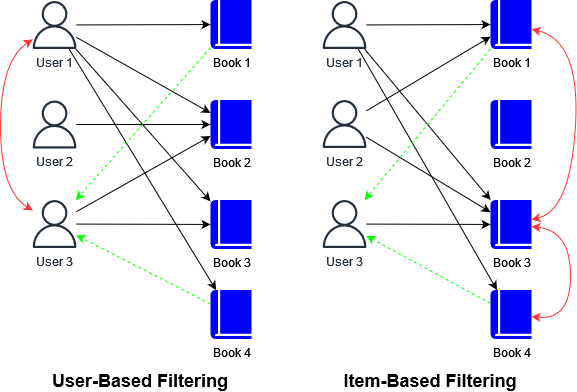
\includegraphics[width=0.9\textwidth]{img/collaborative_example.png}
    \caption{Illustration of Memory-based CF recommendation}
    \label{fig:collaborative_example}
\end{figure}
%
%
When trying to implement this type of recommendation system it is important to consider the key components, which are: 
\begin{itemize}
\item Rating Normalization - adjusts individual user ratings to a standard scale by addressing personal rating habits. Using for example Mean-Centering or Z-Score Normalization. 
\item Similarity Weight Computation - helps to select reliable neighbors for prediction and deciding how much impact each neighbor's rating has. A lot of Similarity measures can be used, such as Correlation-Based Similarity, Mean Squared Difference or Spearman Rank Correlation. 
\item Neighborhood Selection - selects the most appropriate candidates for making predictions based on each unique scenario, eliminating the least likely ones to leave only the best options. \cite{Ning201537}\\
\end{itemize}
%
%
\textbf{Model-based CF}\\
Collaborative filtering systems based on models, also known as Learning-based methods, try to develop a parametric model of the relationships between items and users. These models can capture patterns in the data, which can not be seen in the previous recommendation type. \\
Model-based algorithms do not suffer from memory-based drawbacks and can create prediction over a shorter period of time compared to memory-based algorithms because these algorithms perform off-line computation for training. 
The well-known machine learning techniques for this approach are matrix factorization, clustering and machine learning on the graph \cite{NILASHI2018507}. \\\\
%
%
%
\textbf{Matrix Factorization}\\
In its basic form, matrix factorization characterizes both items and users by vectors of factors inferred from item rating patterns. High correspondence between item and user factors leads to recommendations \cite{5197422}. \\
People prefer to rate just a small percentage of items, therefore the user-item rating matrix, that tracks the ratings people assign to various items, is frequently sparse.\\
In order to deal with this sparsity, matrix factorization (MF) algorithms split the matrix into two lower-rank matrices: one that shows the latent properties of the items and another that reflects the underlying user preferences. These latent representations can be used to predict future ratings or complete the matrix's missing ratings after factorization \cite{Tokala2023}.\\\\
%
%
%
It is important to mention that the effectiveness depends on the ratio of users and items. For example when trying to recommend songs, there are usually way more users than songs and generally, many users listened to the same songs or same genres. Which means like-minded users are found easily and the recommendations will be effective. On the other hand, in a different field for example, when recommending books or articles the systems deals with millions of articles but a lot less users. This leads to less ratings on papers or no ratings at all, so it is harder to find people with shared interests \cite{Beel2016305}.\\








\subsubsection{Content-Based Filtering}
Recommender Systems which are using content-based filtering, review a variety of items, documents and their details. Each product has their own description which is collected to make a model for each item. The model of an item is composed by a set of features representing its content. \\
The main benefit of content-based recommendation methods is that they use obvious item features, making it easy to quickly describe why a particular item is being recommended. \cite{pub.1034486657}\\
This also allows for the possibility of providing explanations that list content features that caused an item to be recommended, potentially giving readers confidence in the system’s recommendations and insight into their own preferences \cite{Mooney2000195}. \\
These profiles for items are different representations of information and users interest about the specific item. \\
The recommendation process basically consists in matching up the attributes of the user profile against the attributes of a content object. \cite{pub.1034486657}\\
%
%
Some additional side information about items can be also useful, where this side information contains additional knowledge about the recommendable items, e.g., in terms of their features, metadata, category assignments, relations to other items, user-provided tags and comments, or related textual content. \cite{Lops2019239}\\\\
The process for recommending items using content-based filtering has 3 different phases and this high level architecture is shown in Fig.~\ref{fig:high_lvl_content_based}.:
\begin{itemize}
\item Content Analyzer - Turns the unstructured information (text) into structured, organized information using pre-processing steps which are basic methods in Information Retrieval, such as feature extraction.
\item Profile Learner - Collects data of the users preference (feedback) that can be either positive information reffering to features which the active user likes or negative ones which the user does not like. After generalization it tries to construct user profiles for later use.
\item Filtering Component - Matches the items for the user, based on the similarities between item representations and user profiles, meaning it compares the features of new items with features in user preferences that are stored in the users profile. \cite{pub.1034486657}
\end{itemize}
%

\begin{figure}[ht]
    \centering
    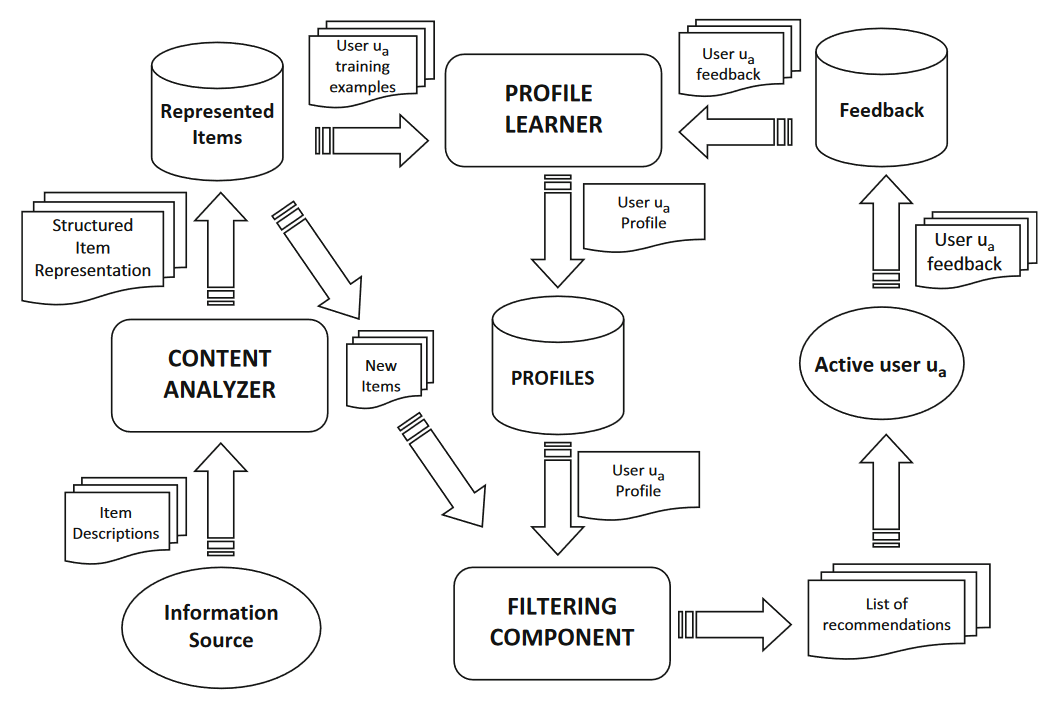
\includegraphics[width=0.9\textwidth]{img/content_based_figure_1.png}
    \caption{High level architecture of a content-based recommender \cite{Musto2022251}}
    \label{fig:high_lvl_content_based}
\end{figure}

The user modeling process has the goal to identify what are the users needs and this can be done 2 ways. Either the system calculates them from the interactions between the user and items through feedback or the user can specify these needs directly by giving keywords to the system, providing search queries \cite{Beel2016305}. \\\\
%
%
\textbf{Feedback}\\
When trying to acquire helpful information or criticism that is given by the user there are 2 separate ways.
The first one is called Explicit Feedback where it is necessary for the user to give item evaluation or actively rate products. Most popular options are gathering like/dislike ratings on items or the ratings can be on a scale either from 1 to 5 or 1 to 10. After the ratings the user can also give comments on separate items. \\
The other way is called Implicit Feedback where the information is collected passively from analyzing the users activities. Some alternatives can be clicks on products, time spent on sites or even transaction history \cite{DeGemmis2015119}.\\\\
%
%
%
\textbf{Advantages and Disadvantages of CB Filtering}
\begin{itemize}
\item User Idependence - meaning the ratings taken into consideration are only provided by the active users to build their own profiles. Collaborative approaches will recommend items based on feedback from other users in the nearest neighborhood.
\item Transparency - explanations for the recommended items can be provided explicitly by listing the content features which were used to get that recommendation. On the other hand Collaborative systems are considered black boxes, where explanations are based on similar tastes of different users.
\item New Item - when a new item is added to the system, the Content-based method is capable of recommending it from the set features and its content. This is not possible for the Collaborative method which needs feedback for the new item to be able to recommend it.
\item Limited Content Analysis - because the system can only analyze a certain number of features and can miss important aspects such as aesthetics or other multimedia information. Also, systems based on string matching approach can suffer from problems such as synonymy, polysemy or multi-word expressions.
\item Over-Specialization - the user will mostly be recommended things similar to what they already liked, which drawback is called 'lack of serendipity'. For example, if the user only rated action movies, then the system would not recommend other genres, which limits the chance of recommending items with novelty or surpise. \cite{DeGemmis2015119}\\
\end{itemize}
%
%
%
%
\textbf{Semantic approaches in CB Recommendation}\\
In short, Semantics refer to interpretation of meaning in language, words and symbols. Using semantic techniques the represantations of items and user profiles shift from keyword-based to concept-based ones.  With these represantations it is possible to give meaning to information expressed in natural language and to get a deeper understanding of the information presented by textual content.\\
Content-based recommendations can adopt two different approaches based on how the semantics are derived and applied:
\begin{itemize}
\item \textbf{Top-Down Semantic Approaches} use an external knowledge to improve the representation of the items and users. This external knowledge can be: ontological resources, encyclopedic knowledge (ESA, BabelNet) and the Linked Open Data cloud. For example the \textbf{Ontology} is a structured description that shows how different parts of a system depend on each other and how they are connected. It organizes key concepts in a specific domain into a hierarchy, which can explain their relationships and the characteristics of each concept. It can help to understand how specific examples of these concepts behave and how they are related \cite{pub.1090632691}.
%
\item \textbf{Bottom-Up Semantic Approaches} use implicit semantic representation of items and user profiles, where the meanings of terms are assumed by analyzing its usage. They rely on the distributional hypothesis: "words that occur in the same context tend to have similar meanings". Without a predefined structure, this approach analyzes the words co-occurrence with other words, larger texts or documents using Discriminative Models.\cite{DeGemmis2015119}
\end{itemize}
%
%
The semantic approaches can be further categorized by the source of knowledge used to extract meaning, which are \textbf{Endogenous Semantics} and \textbf{Exogenous Semantics}.
In the first case, the semantics is obtained by exploiting unstructured data, and is directly inferred from the available information. Different techniques for these Implicit Semantics Representations are for example the Term Frequency - Inverse Document Frequency (TF-IDF) weighting, or the Distributional Semantics Models (DSM) such as Explicit Semantics Analysis (ESA), Random Indexing or Word Embedding Techniques.
Word embedding technology can reflect the semantic information of words to a certain extent. The semantic distance between words can be calculated by word vectors. Commonly used word vectors are based on for example Word2vec or Fasttext models \cite{Huang2023}.\\
%
In the second, the semantics comes from the outside, since it is obtained by mining and exploiting data
which are previously encoded in structured and external knowledge sources. For these Explicit Semantics Representations there are also different techniques like Linking Item Features to Concepts using Word Sense Disambiguation (WSD) or using Entity Linking, or Linking Items to Knowledge Graphs using Ontologies or Linked Open Data (LOD). \cite{Musto2022251} \\
The LOD cloud is a huge decentralized knowledge base where researchers and organizations publish their data in Resource Description Framework (RDF) format and adopt shared vocabularies, in order to express and interlink the data to each other \cite{Musto2017405}.
%
%
%
%\clearpage
\subsubsection{Knowledge Graphs}
Knowledge graph is a knowledge base that uses a graph-structured data model. It is a graphical database which contains a large amount of relationship information between entities and can be used as a convenient way to enrich users and items information \cite{Imene2022488}.\\
%
The idea is that attributes of users and items are not isolated but linked up with each other, which forms a knowledge graph (KG). Incorporating a Knowledge Graph into recommendations can help the results in ways like:
\begin{itemize}
\item The rich semantic relatedness among items in a KG can help explore their latent connections and improve the precision of results.
\item The various types of relations in a KG are helpful for extending a user’s interests reasonably and increasing the diversity of recommended items.
\item KG connects a user’s historically-liked and recommended items, thereby bringing explainability to recommender systems. \cite{Wang20193307}
\end{itemize}
%
Basically a knowledge graph is a directed graph whose nodes are the entities and the edges are the relations between them. They are usually defined as triplets with a head entity, tail entity and a relationship connecting them. The graphs have detailed supporting information which is background knowledge of items and their relations amongst them. The facts of items are organized in those triplets like (Ed Sheeran, IsSingerOf, Shape of You), which can be seamlessly integrated with user-item interactions. This interaction data is usually presented as a
bipartite graph \cite{pub.1120733877}. \\
The crucial point to leverage knowledge graphs to perform item recommendations is to be able to effectively model user-item relatedness from this rich heterogeneous network \cite{Palumbo201732}. \\ 
%
%
\begin{figure}[h!]
    \centering
    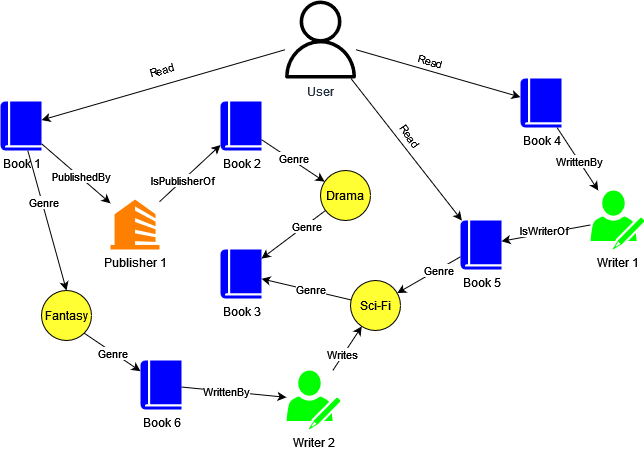
\includegraphics[width=1\textwidth]{img/knowledge_graph_example.png}
    \caption{Illustration of KG-aware recommendation}
    \label{fig:knowledge_graph_example}
\end{figure}
%
%
\newpage{}
Recommendation methods based on knowledge graphs can be practically categorized into two different types which are Path-based and Embedding-based methods. Where the \textbf{Embedding-based} method uses knowledge graph embedding (KGE) techniques trying to learn how to represent users and items. This method uses representation learning to find connections implicitly, rather than using user preferences. Models such as TransE, TransR and TransH build entity and relation embeddings by regarding a relation as translation from head entity to tail entity. These models simply put both entities and relations within the same semantic space. \cite{pub.1148917041}\\
The \textbf{Path-based} method focuses on enhancing the connections called meta-paths that link the users and items, showing how similar they are \cite{Yang20229308}. 
%
\subsubsection{Hybrid Approaches}
The Hybrid recommender systems try to combine two or more recommendation techniques to get to better performance and accuracy. The most common approach is to have a collaborative filtering technique combined with some other technique to try to avoid the ramp-up problem.
The ramp-up problem actually means two problems, which are "New User" and "New Item" problems (hard to categorize with few ratings).\\
Different types of hybrid recommender systems exist, here are the following hybdirds listed \cite{Burke2002331}:
\begin{itemize}[label=--]
\item \textbf{Weighted hybrid} - initially gives equal weight to all available recommendation techniques in the system. Gradually adjusts the weighting based on wether the predicted user ratings are confirmed or discomfirmed. The recommended items score is computed from the results.
\item \textbf{Switching hybrid} - the system switches between recommendation techniques based on some criterion. The advantage is that the system can adapt to the strengths and weaknesses of the different recommendation methods it combines.
\item \textbf{Mixed hybrid} - recommendations from more than one technique are presented together at the same time. 
\item \textbf{Feature combination} - for example in a content / collaborative merger the system treats the collaborative information as an additional feature data and uses content-based techniques over this enhanced dataset.
\item \textbf{Cascade hybrid} - one recommender produces a coarse ranking of candidates and than the other refines the recommendations given by the first one. The second step only focuses on the items given by the first step and not all items in the dataset.
\item \textbf{Feature augmentation} - one technique produces a rating of an item and that information is then incorporated into processing the next recommendation technique. The features used by the second recommender include the output of the first one (like ratings).
\item \textbf{Meta-level hybrid} - combines two techniques by using the model generated by one as the input for the other, meaning the entire model becomes the input.\\
\end{itemize}
%
%
%
%%%%%%%%%%%%%%%%%%%%%%%%%%%%%%%%%%%%%%%%%%%%%%
%
\subsection{Difficulties related to Recommendation Systems}
All types of recommendation systems encounter significant challenges which they have to face and issues they have to solve. Here are some main challenges:
%
\begin{itemize}
\item Cold-start problem - arises when making recommendations to new users and/or items for which the available information is limited. As a result, the recommendations offered in such cases tend to be of poor quality and lack usefulness.\cite{Al-Hassan2024a}
\item Data sparsity - when recommender systems use large datasets, the user-item matrix used for filtering can be sparse, which leads to worse performance of recommendations.
\item Scalability - as the number of users and items increases, so does the complexity of the algorithms used for recommending items.
\item Diversity - helps to discover new products, but some algorithms may accidentally do the opposite, which can also lead to lower accuracy in the recommendation process. \cite{pub.1072601078}
\item Privacy - because the information collected by the system usually includes sensitive information that users wish to keep private, users may have a negative impression if the system knows too much about them.
\item Serendipity - sometimes can be useful, but if the result of the recommendation system only has
serendipitous items and does not have related items, user may think that the system is not reliable. \cite{Aymen2022896}
%\item Exploration vs. Exploitation
\end{itemize}
%
%%%%%%%%%%%%%%%%%%%%%%%%%%%%%%%%%%%%%%%%%%%%%%
%
\subsection{Evaluation of Recommendation Systems}
When trying to choose which recommendation approach is the best, first it is important to know the use case for the specific system. \\
The process of finding the most appropriate algorithm for the specific goal typically is based on experiments, comparing the performance of a number of candidate recommenders. Comparing the performance of an algorithm is mostly performed by using some evaluation metric, which usually uses numeric scores, that provides ranking of the compared algorithms. \\
For measuring the accuracy of predictions of the algorithm three classes of measurements are defined, which are \cite{Gunawardana2022547}:
\begin{itemize}
\item \textbf{Measuring Ratings Prediction Accuracy} wishes to measure the accuracy of the system's predicted ratings. The following metrics can be used in such situation: Root Mean Squared Error (RMSE), Mean Absolute Error (MAE), Normalized RMSE, Normalized MAE, Average RMSE, Average MAE.
\item \textbf{Measuring Usage Prediction} tries to recommend to users items that they may use, with the following metrics: Precision, Recall (True Positive Rate), False Positive Rate (1 - Specificity), F-measure, Area Under the ROC Curve (AUC).
\item \textbf{Ranking Measures} are not predicting an explicit rating, but rather are ordering items according to the user's preferences. This can be done Using a Reference Ranking like Normalized Distance based Performance Measure (NDPM), Average Precision (AP) correlation, Spearman's rank correlation coefficient, Kendall's rank correlation coefficient or using Utility-Based Ranking such as Normalized Discounted Cumulative Gain (NDCG), Discounted Cumulative Gain (DCG) or Average Reciprocal Hit Rank (ARHR). Other than that there is also Online Evaluation of Ranking.
\end{itemize}
%
%
%
The previously mentioned metrics mostly need the feedback from the users, wether it is from ratings or interaction, the metrics are calculated comparing the recommended list with the users data, so knowing which user interacted with which item shows wether the recommendation was accurate or not. However, not all users are trying to use the recommendation engine just for the most accurate predictions, but they might be more interested in other properties of the recommender system like \cite{Gunawardana2022547}:
\begin{multicols}{3}
\begin{itemize}
\item Coverage
\item Confidence
\item Trust
\item Novelty
\item Serendipity
\item Diversity
\item Utility
\item Risk
\item Robustness
\item Privacy
\item Adaptability
\item Scalability
\end{itemize}
\end{multicols}
%
%
%
In the domain of scientific publications, where users are relatively few with respect to the available documents, information needs and interests easily change in an unpredictable way over time due to evolving professional needs, there is also no advertising pushing new items.
%, and the long tail of infrequently read articles may contain the so-called sleeping beauties, that are documents containing extremely relevant results, but that remains unknown to most researchers for a very long time. \\
The Content-based approach does not require particular assumptions over the size and the activity of the user base. It does not penalize items that have less ratings or are less frequently consumed by many users as long as enough metadata are available, which even allows detailed explanations. These advantages over Collaborative Filtering techniques make this approach particularly attractive to the purpose of providing recommendation in the domain of scientific publications \cite{De_Nart201484}. 
%
%
\subsection{Related Works}
%\cite{Beel2016305} - 2016 - more than half recommenders are content based
%\cite{Silveira2019813} - 2019 - good metrics
%\cite{Zangerle2023} - ACM - 2022
%\cite{Aymen2022896} - scientific paper recommender 2022 - review of other works
%
Several works have explored the application of content-based recommendation systems in the context of digital libraries and book recommendations. Authors in \cite{Beel2016305} conducted a comprehensive survey on recommender systems in digital libraries, highlighting that more than half of the systems used content-based filtering as their core technique due to the lack of explicit user feedback in academic datasets and the rich textual metadata available for papers and books. Their approach emphasized keyword-based similarity measures, often relying on TF-IDF or simple cosine similarity to recommend research articles.

Authors in \cite{Zangerle2023} presented a structured framework for the evaluation of recommender systems, called the Framework for Evaluating Recommender Systems (FEVR). 
Their work summarizes insights on how to evaluate recommender systems and organizes them into clear categories, such as evaluation goals, methods, data used, and metrics. The authors argue that all these aspects should be considered together to get meaningful and reliable results. The FEVR framework helps researchers design solid and well-rounded evaluation setups that fit different types of recommender systems.

Authors in \cite{Silveira2019813} surveyed and formalized six key evaluation concepts: utility, novelty, diversity, unexpectedness, serendipity, and coverage. They provided standardized notations and levels of user dependency. Their work critically reflects on how different metrics are connected, categorizing some as user-dependent (e.g., utility, unexpectedness) and others as user-independent (e.g., diversity, coverage). Moreover, they discuss how many metrics overlap in intent and application, and propose that future evaluation frameworks should better align with actual user satisfaction through hybrid online-offline methodologies.

In contrast to these earlier systems, the approach in this work includes Content-based filtering and for similarity measuring using Cosine Similarity applied to different text representation techniques, from traditional TF-IDF and BoW to contextual embeddings like BERT. The evaluation is based on user-independent metrics such as similarity, coverage, diversity, confidence because of the absence of user feedback and user-item interaction. 



%%%%%%%%%%%%%%%%%%%%%%%%%%%%%%%%%%%%%%%%%%%%%%%%%%%
%\begin{itemize}
%\item 
%\item 
%\end{itemize}


\clearpage
%
%
%\subsection{Hypotheses}
%A hypothesis is a specific description or prediction to define the evaluation's goal. It serves as the foundation for experiments showing the direction for testing and analyzing the results. The more precise the hypothesis, the clearer the setup of the evaluation.\\\\
%\textbf{Hypothesis 1:} Algorithms with contextual embeddings (BERT, FastText) will achieve higher \textbf{Usage Prediction} scores than simpler frequency-based methods (TF-IDF, BM25).\\
%%
%\textbf{Hypothesis 2:} Probabilistic models (LDA) will have higher \textbf{Coverage} compared to neural embedding techniques (Word2Vec, BERT), as they can better generalize relationships across sparse datasets.\\
%%
%\textbf{Hypothesis 3:} Transformer-based algorithms (BERT) will outperform other methods on \textbf{Ranking Measures} like NDCG because they leverage bidirectional encoding to better understand query-item relevance.\\
%%
%\textbf{Hypothesis 4:} Word2Vec and FastText will generate more \textbf{Diverse} recommendations than probabilistic or frequency-based methods, as their embeddings capture subtler relationships between less frequently co-occurring terms.\\
%%
%\textbf{Hypothesis 5:} GloVe and LSA will recommend items with higher \textbf{Novelty} scores compared to algorithms like BM25 or TF-IDF, as they infer latent relationships beyond direct term matches.\\
%%
%\textbf{Hypothesis 6:} BERT and Word2Vec will provide the highest \textbf{Confidence} in recommendations, as their embeddings are more precise and context-aware, resulting in smaller prediction uncertainty.\\




\section{Implementation Proposal}
% 5-10 Pages \\\\
Drawing from the theoretical foundation in the second section, this section proposes a practical framework for evaluating different text representation algorithms tested on recommending books from digital library datasets based on textual metadata and full-text features. We also describe the dataset we will be working with. The proposal includes a detailed explanation of our experiment, along with the rationale behind our choices of specific text represenation methods.
%
%
%
\subsection{Dataset Analysis}
The main objective of this project is to compare different recommendation algorithms for digital library datasets. To support this, a collection of academic books extracted from the digital library will be used. 
%converted from PDF format into structured JSON files, 
These books have the text segmented into individual sentences, paragraphs and pages. The experiments will primarily focus on paragraph-level recommendations, as suggesting relevant content based on a single paragraph can be a valuable feature for navigating academic materials in a digital library.
%
\begin{figure}[H]
    \centering
    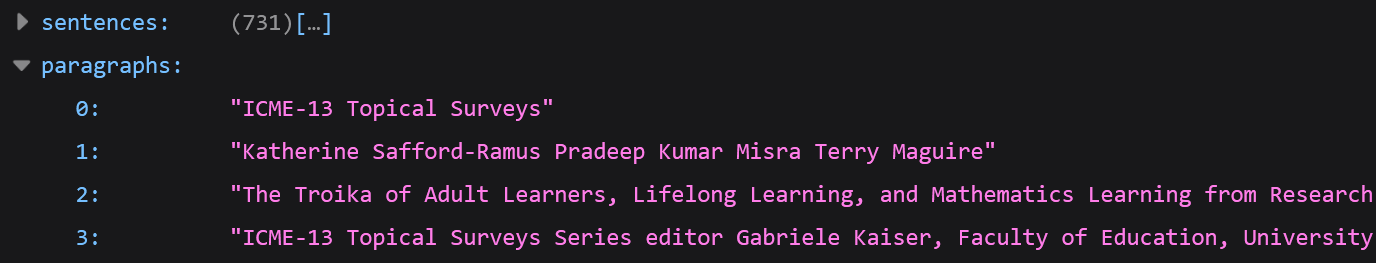
\includegraphics[width=1\textwidth]{img/json_example2.png}
    \caption{Example of extracted book paragraphs}
    \label{fig:extracted_paragraph_example}
\end{figure}
%
In addition to this dataset, a second dataset will be used to test the algorithms on simpler and more general types of text. This dataset, from Goodreads, contains book metadata and short descriptions for a wide range of genres including fantasy, comedy, romance, and others. Unlike the academic content of the first dataset, this one includes more casual, narrative-driven books, which helps test the algorithms’ performance on short-form and less formal text.
%
\begin{figure}[H]
    \centering
    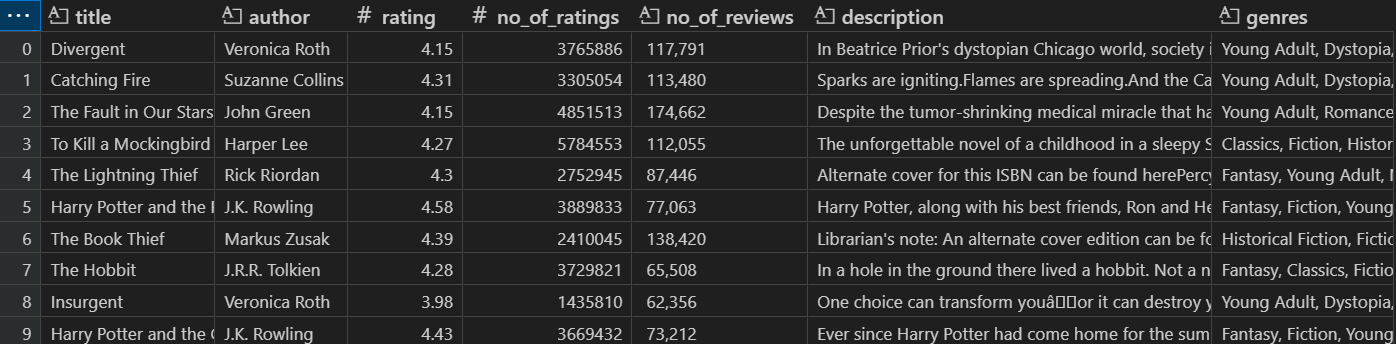
\includegraphics[width=1\textwidth]{img/rating_data_example2.png}
    \caption{Example of book descriptions dataset \cite{goodreads_kumar_2022}}
    \label{fig:book_description_dataset_example}
\end{figure}
%
By using 2 different datasets in experiments it will ensure that the evaluation covers specialized and general-purpose recommendation use cases. Basic preprocessing such as tokenization, removal of special characters, and optional stopword filtering will be applied prior to embedding.
%
%
%
\subsection{Text Representation Methods}
In order to build a robust and interpretable content-based recommendation system, a diverse set of seven text representation models is selected: 
\begin{itemize}
\item TF-IDF
\item Bag of Words (BoW)
\item Latent Semantic Analysis (LSA)
\item GloVe
\item FastText
\item BERT
\item E5
\end{itemize}
%
These models chosen represent a broader spectrum of natural language processing techniques, ranging from classical statistical approaches to modern deep learning-based embeddings.
This selection has 2 goals. First, to evaluate how different levels of semantic understanding affect recommendation quality and second, to establish clear baselines against which newer models could be compared to later. Each model has its own strengths that help us understand and use text similarity in recommendation tasks more effectively.\\
%
%
Below is an overview of the different methods that will be used for text representation, highlighting their methodology and key characteristics:
\begin{enumerate}
\item \textbf{TF-IDF (Term Frequency - Inverse Document Frequency)}\\
TF-IDF is selected as a well-established and interpretable baseline for measuring textual similarity. It captures term importance based on document frequency and enables fast similarity computation using sparse vectors.
TF-IDF creates two scores that are interrelated, trying to figure out the relevancy of a given term (word) to a document given a larger body of documents. TF means how often a given word occurs in the given document, because words that occur frequently are probably more important. DF means how often the given word occurs in an entire set of documents, but this does not have to mean the word is important, it just shows common words that appear everywhere. So using Inverse DF shows how often the word appears in a document, over how often it appears everywhere \cite{pub.1022525812}.


\item \textbf{BoW (Bag of Words)}\\
BoW is probably the most simple method selected here, it provides a valuable lower bound for comparison. It does not consider word order and semantics, making it a good contrast point to evaluate the improvements introduced by more complex models.
BoW creates a set of vectors containing the count of word occurrences in the document. Unlike TF-IDF, BoW just counts the occurrences of unique words and puts them in its vocabulary so each word becomes a feature or dimension. Each document is represented as a vector based on the frequency of words from the vocabulary. The term-document matrix represents the documents as rows and the unique words as columns with cells showing frequency.
 

\item \textbf{LSA (Latent Semantic Analysis)}\\
LSA extends TF-IDF by applying dimensionality reduction through Singular Value Decomposition (SVD) to uncover hidden patterns and relationships between terms and documents. This technique helps capture the underlying semantic structure of the text. By decomposing the term-document matrix into three smaller matrices representing topics, terms, and documents LSA identifies latent topics and represents documents in a lower-dimensional semantic space. \cite{Bergamaschi2015247}.


\item \textbf{GloVe (Global Vectors for Word Representation)}\\
GloVe is included as a pretrained static word embedding model that represents words as fixed-size vectors based on how often they appear together in a large text corpus. It builds a co-occurrence matrix where rows represent the words, columns represent the context words and each cell contains the frequency with which the word and context word co-occur within a specified window to learn the relationships between words, allowing it to capture their meanings and similarities. GloVe helps to test how well combining individual word vectors can represent the meaning of a full document.


\item \textbf{FastText}\\
FastText enhances traditional word embeddings by incorporating subword information, allowing the model to generate embeddings even for rare or complex words. FastText breaks words into character n-grams and learns embeddings for these subwords. It can handle words that are out of the vocabulary, because it models character n-grams and not words. For output it produces dense, fixed-length word vectors that have the additional subword information \cite{Yan2024}.


\item \textbf{BERT (Bidirectional Encoder Representations from Transformers - SentenceTransformer)}\\
BERT represents the state-of-the-art in contextual language modeling. Unlike the other models, BERT produces embeddings that consider the full sentence context, allowing it to distinguish between different meanings of the same word depending on usage. It uses attention mechanisms to model relationships between all words in a sentence allowing bidirectional encoding. \cite{Lim2025}

\item \textbf{E5 (Embedding-based Encoder for Information Retrieval)}\\
E5 is a transformer-based model, designed specifically for dense retrieval and semantic similarity tasks. Similar to BERT, it produces contextual embeddings at the sentence level, capturing the underlying meaning of text rather than relying on surface-level token matches. E5 excels in matching short texts such as questions, passages, or document segments based on semantic relevance.

%\item \textbf{LDA (Latent Dirichlet Allocation)}\\
%Is a generative model for document collections, unlike LSA, LDA is a probabilistic Topic Model, which decomposes a conditional term by the document porbability distribution into two different distributions, the term by topic distribution and the topic by document distribution. After running LDA, each document is represented as a topic distribution, i.e., a vector of probabilities indicating the degree to which each topic is present in the document. 

%\item \textbf{Word2Vec}\\
%Is a neural network-based algorithm that generates dense vector representations for words (embeddings). The neural network uses one hidden layer to create the embeddings, it comes in two main architectures. Using Continuous Bag of Words (CBoW) which predicts a target word based on the words around it, or using Skip-Gram which predicts the context words given a target word. The output is a vector for each word in the vocabulary.
%
%\item \textbf{Doc2Vec}\\
%Is an extension of Word2Vec also being a neural network-based algorithm, but is designed to generate dense vector representations for entire documents or sentences, not just words. It enhances the Word2Vec by adding a document vector, which represents the unique context of an entire document. Here are also two main architectures, the first is the Distributed Memory Model of Paragraph Vectors (PV-DM) which predicts a word within a context using the surrounding words and a document vector, and the second is the Distributed Bag of Words (PV-DBOW) which instead of predicting a word using context, it predicts context words using the document vector alone. For output each document is represented by a fixed-length dense vector, regardless of its size or content.

%\item \textbf{BM25 (Best Match 25)}\\
%Is a ranking function that builds on the TF-IDF model. It ranks a set of documents based on the query terms appearing in each document, not considering their proximity within the document.
\end{enumerate}
%
By including models from these various categories (statistical, latent, word-level embeddings, and contextual transformer-based representations) the experimental design ensures a wider comparison across different levels of linguistic representation.
%
\subsection{Experiment Types}
%
Experimenting with recommendations can be done in different ways. Here are the types of experiments to test the algorithms:
{
\renewcommand{\arraystretch}{1.5}
\begin{table}[h!]
\centering
\begin{tabular}{p{3cm}|p{10cm}}
\hline
\textbf{Type} & \textbf{Description} \\
\hline
Offline & Method: simulation of user behavior based on past interactions \\
        & Task: defined by the researcher, purely algorithmic \\
        & Repeatability: evaluation of an arbitrary number of experiments possible at low cost \\
        & Scale: large dataset, large number of users \\
        & Insights: quantitative, narrow \\
\hline
User Study & Method: user observation in live or laboratory setting \\
           & Task: defined by the researcher, carried out by the user \\
           & Repeatability: expensive \\
           & Scale: small cohort of users \\
           & Insights: quantitative and/or qualitative \\
\hline
Online & Method: real-world user observation, online field experiment \\
       & Task: self-selected by the user, carried out by the user \\
       & Repeatability: expensive \\
       & Scale: large \\
       & Insights: quantitative and/or qualitative \\
\hline
\end{tabular}

\caption{Overview of Experiment Types \cite{Zangerle2023}}
\end{table}\\
}
%
%
\textbf{Offline experiments} are the most popular experiment type. They aim to compare different recommendation algorithms and settings and they do not require any user interaction and may be considered system-centric \cite{Zangerle2023}. 
The \textbf{offline evaluation} method will be adopted, as the goal is to test and compare recommendation algorithms without relying on actual user interaction or feedback. This provides a practical way to test the system without users and could be repeated as many times as needed for system-centric experimentation.
%
%\begin{table}[h!]
%\centering
%\renewcommand{\arraystretch}{2}
%{\large
%\begin{tabular}{|m{0.03\textwidth}|m{0.5\textwidth}|}
%\hline
%\textbf{\#} & \textbf{Feature Extraction Algorithms} \\ \hline
%1            & TF-IDF  \\ \hline
%2            & BoW  \\ \hline
%3            & GloVe \\ \hline
%4            & LSA \\ \hline
%5            & LDA  \\ \hline
%6            &  Word2Vec  \\ \hline
%7            & Doc2Vec   \\ \hline
%8            &  BERT  \\ \hline
%9            & FastText \\ \hline
%10           & BM25  \\ \hline
%\end{tabular}
%}
%\caption{Feature Extraction Methods}
%\label{table:feature_extraction}
%\end{table}
%
%
%
% \vspace*{2\baselineskip}
%\pagebreak{}
%\subsection{Descriptions of Similarity and Distance Measures:}
%Similarity and distance measures are critical for comparing items and identifying the most relevant recommendations. These measures quantify how closely two data points—such as the input items and the recommended items features—relate to each other in a multi-dimensional space. Different measures are suited for varying data types and use cases, impacting the effectiveness of the recommendation algorithm. Below are descriptions of the similarity and distance measures that will be used, each with its unique approach to comparing items or features:
%%
%%
%\begin{table}[H]
%\centering
%\renewcommand{\arraystretch}{1.5}
%{\large
%\begin{tabular}{|c|p{0.25\textwidth}|p{0.60\textwidth}|}
%\hline
%\textbf{\#} & \textbf{Measure} & \textbf{Description} \\ \hline
%1 & Cosine Similarity & Measures the cosine of the angle between two vectors in a multi-dimensional space. Ranges from -1 to 1 (-1 means completely opposite, 1 means completely similar). \\ \hline
%2 & Euclidean Distance & Calculated as the square root of the sum of squared differences between corresponding dimensions. It shows the straight-line distance between two points. \\ \hline
%3 & Jaccard Similarity & Measures the similarity between two sets by dividing the size of their intersection by the size of their union. \\ \hline
%4 & Manhattan Distance & Calculates the sum of the absolute differences between the coordinates of two points. \\ \hline
%5 & Pearson Correlation & Measures the linear correlation between two variables. Ranges from -1 to 1 (-1 means negative correlation, 1 means positive correlation, 0 means no linear relationship). \\ \hline
%6 & Bray-Curtis Distance & Measures the dissimilarity between two vectors as the sum of absolute differences divided by the sum of all values. \\ \hline
%7 & Canberra Distance & Calculated as the sum of absolute differences divided by the sum of the absolute values of the components. It is a weighted version of Manhattan Distance. \\ \hline
%8 & Minkowski Distance & Generalizes the Euclidean and Manhattan distances. It is controlled by a parameter p. \\ \hline
%9 & Mahalanobis Distance & Measures the distance between a point and a distribution, considering correlations between variables. \\ \hline
%10 & Wasserstein Distance & Measures the cost of transforming one probability distribution into another. \\ \hline
%\end{tabular}
%}
%\caption{Similarity and Distance Measures}
%\label{tab:similarity_measures}
%\end{table}
%
%
%
% \textbf{Combinations of Algorithms with Measures:}\\ %%%%%%%%%%%%%
%
%
%
%
\subsection{Conceptual Proposal}
\begin{enumerate}
    \item \textbf{Loading raw data from JSON files}
    \begin{itemize}
        \item Paragraphs will be extracted from academic books into a structured format, with book and paragraph index
    \end{itemize}

    \item \textbf{Including an additional dataset of book descriptions}
    \begin{itemize}
        \item A second dataset containing book metadata and textual descriptions (from Goodreads) will be used
        \item This dataset includes books from various genres such as fantasy, comedy, and romance, with the goal of testing on short-form, non-academic content
    \end{itemize}

    \item \textbf{Preprocessing and organization}
    \begin{itemize}
        \item Both datasets will be organized in DataFrames for consistent handling
        \item Text will be cleaned and normalized to prepare it for embedding
    \end{itemize}
    
    \item \textbf{Implementation of the recommendation algorithm}
    \begin{itemize}
        \item A pipeline will be developed for generating recommendations based on paragraph-to-paragraph and description-to-description similarity
        \item The system will support multiple text representation techniques
    \end{itemize}

    \item \textbf{Integration of different text representation methods}
    \begin{itemize}
	\item TF-IDF (Term Frequency–Inverse Document Frequency)
	\item LSA (Latent Semantic Analysis)
	\item BoW (Bag of Words)
	\item FastText (Facebook's FastText Word Embeddings)
	\item GloVe (Global Vectors for Word Representation)
	\item BERT (Bidirectional Encoder Representations from SentenceTransformers)
	\item E5 (Embedding-based Encoder for Information Retrieval from SentenceTransformers)
    \end{itemize}


    \item \textbf{Running experiments and storing results}
    \begin{itemize}
        \item Each model will be executed independently on both datasets
        \item Top-N recommendations will be generated for selected input texts
    \end{itemize}

    \item \textbf{Evaluation of recommendations}
    \begin{itemize}
        \item Evaluation will be based on metrics
        \item Time and memory usage will be tracked to compare algorithm performance
    \end{itemize}


\end{enumerate}
%


%The following diagram summarizes the overall flow of the proposed system:




%\begin{figure}[h!]
%\centering
%\begin{tikzpicture}[
%    node distance=1.2cm and 0.9cm,
%    every node/.style={draw, align=center, rounded corners=5pt, minimum width=2.3cm, minimum height=1cm},
%    smallnode/.style={draw, align=center, rounded corners=4pt, minimum width=1.9cm, minimum height=0.9cm},
%    arrow/.style={-{Latex}, thick}
%]
%
%% Representation model nodes
%\node[smallnode] (tfidf) {TF-IDF};
%\node[smallnode] (bow)   [right=of tfidf] {BoW};
%\node[smallnode] (lsa)   [right=of bow]   {LSA};
%\node[smallnode] (glove) [right=of lsa]   {GloVe};
%\node[smallnode] (fasttext) [right=of glove] {FastText};
%\node[smallnode] (bert)  [right=of fasttext] {BERT};
%\node[smallnode] (e=5)  [right=of bert] {E5};
%
%% Preprocessing - centered between tfidf and bert
%\node (preprocess) [above=1.5cm of $(tfidf)!0.5!(bert)$] {Preprocessing and Cleaning};
%
%% Input datasets
%\node (json) [above left=0.8cm and 1.2cm of preprocess] {JSON Dataset\\(paragraphs)};
%\node (goodreads) [above right=0.8cm and 1.2cm of preprocess] {Goodreads Dataset\\(descriptions)};
%
%% Recommendation pipeline
%\node (pipeline) [below=2cm of $(lsa)!0.5!(glove)$] {Recommendation Pipeline};
%\node (results) [below=of pipeline] {Top-N Results};
%\node (evaluation) [below=of results] {Evaluation\\(Similarity, Coverage, etc.)};
%
%% Arrows from data sources
%\draw[arrow] (json.south) -- ++(0,-0.4) -| (preprocess);
%\draw[arrow] (goodreads.south) -- ++(0,-0.4) -| (preprocess);
%
%% Arrows from preprocessing to models
%\draw[arrow] (preprocess) -- (tfidf);
%\draw[arrow] (preprocess) -- (bow);
%\draw[arrow] (preprocess) -- (lsa);,
%\draw[arrow] (preprocess) -- (glove);
%\draw[arrow] (preprocess) -- (fasttext);
%\draw[arrow] (preprocess) -- (bert);
%
%% Arrows from models to pipeline
%\draw[arrow] (tfidf) |- (pipeline);
%\draw[arrow] (bow)   |- (pipeline);
%\draw[arrow] (lsa)   -- (pipeline);
%\draw[arrow] (glove) -- (pipeline);
%\draw[arrow] (fasttext) |- (pipeline);
%\draw[arrow] (bert)  |- (pipeline);
%
%% Downstream arrows
%\draw[arrow] (pipeline) -- (results);
%\draw[arrow] (results) -- (evaluation);
%
%\end{tikzpicture}
%\caption{Conceptual flow of the proposed recommendation system with multiple text representation methods}
%\label{fig:concept_flow}
%\end{figure}


%%%%%%%%%%%%%%%%%%%%%%%%%%%%%%%%%%%%%%%%%
%\begin{figure}[h!]
%\centering
%\begin{tikzpicture}[
%    node distance=1.5cm and 1.5cm,
%    every node/.style={draw, align=center, rounded corners=5pt, minimum width=3.5cm, minimum height=1.2cm},
%    arrow/.style={-{Latex}, thick}
%]
%
%% Nodes
%\node (datasets) {Input Datasets\\JSON (paragraphs)\\Goodreads (descriptions)};
%\node (preprocess) [below=of datasets] {Preprocessing and Cleaning};
%\node (textrep) [below=of preprocess] {
%    Text Representation Models\\
%    \scriptsize TF-IDF, BoW, LSA, GloVe, FastText, BERT, E5
%};
%\node (pipeline) [below=of textrep] {Recommendation Pipeline};
%\node (results) [below=of pipeline] {Top-N Results};
%\node (evaluation) [below=of results] {Evaluation\\(Similarity, Coverage, etc.)};
%
%% Arrows
%\draw[arrow] (datasets) -- (preprocess);
%\draw[arrow] (preprocess) -- (textrep);
%\draw[arrow] (textrep) -- (pipeline);
%\draw[arrow] (pipeline) -- (results);
%\draw[arrow] (results) -- (evaluation);
%
%\end{tikzpicture}
%\caption{Simplified flow of the recommendation system}
%\label{fig:simplified_concept_flow}
%\end{figure}




















%
%
% Tokenization, stopword removal, and optional stemming/lemmatization\\\\
%
%
%\newpage{}
%\textbf{Evaluation of Recommender Systems - Objectives and Design Space}
%\begin{figure}[h!]
%    \centering
%    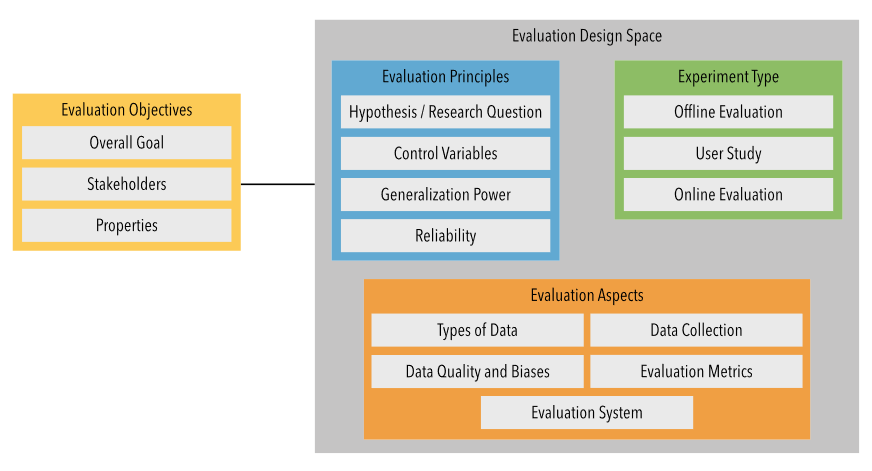
\includegraphics[width=0.9\textwidth]{img/evaluation_figure.png}
%    \caption{Evaluation of Recommender Systems: objectives and design space \cite{Zangerle2023}}
%    \label{fig:evaluation}
%\end{figure}
%





%%%%%%%%%%%%%%%%%%%%%%%%%%%%%%%%%%%%%%%%%%%%%%%%%%%

\clearpage{}
\section{Implementation}
% 3,4,5 Pages\\
This section describes how the proposed system was implemented in practice. It outlines the data preparation process, integration of multiple text representation methods, the overall recommendation pipeline and the development environment.\\
The system was implemented using the \textbf{Python} programming language, which is widely adopted in the fields of data science and machine learning. For data preparation and experimentation, the \textbf{Jupyter Notebook} environment was used. This way the development was interactive with  step-by-step testing of individual components during preprocessing and exploration of various recommendation models.\\
While the notebooks were used locally for developing and testing the recommendation logic, the final recommendation system was implemented as a collection of structured Python scripts. These scripts were executed on a \textbf{Google Cloud Virtual Machine (VM)} configured with 8 vCPUs, 32 GB of RAM, and a dedicated NVIDIA L4 GPU. 
This cloud-based deployment enabled efficient GPU-accelerated execution of models and ensured clean, uninterrupted \textbf{multiprocessing-based resource tracking} across CPU, memory, and GPU usage. \\
Each model was tested in ten evaluation runs using this setup, with results logged for further evaluation. Then the evaluation itself was carried out in a separate Jupyter Notebook, executed locally, where the recommendation results from the VM runs were collected and visualized.

\subsection{Extracting Information and Building a Dataset}
First, the books were extracted from the digital library and stored as individual JSON files. Each file contained the entire data of a single book, further segmented into sentences, pages, and paragraphs for flexibility in experimentation. These JSON files were loaded and parsed into \textit{Pandas DataFrames} for easier handling and segmentation into paragraphs. The processed data was then exported into CSV files and a dataset of 45,461 paragraphs was created. 
The average paragraph length was approximately 60-70 words, with the longest paragraph consisting of 2000 words.\\
In addition to the extracted book paragraphs, a publicly available dataset titled \textit{Books Details Dataset}, which was scraped from Goodreads \cite{goodreads_kumar_2022} was also used in the experiments. This dataset includes metadata for over 13,000 books, such as title, author, genres, ratings, and textual descriptions. The dataset contains entries with descriptions averaging approximately 160 words. These summaries were treated similarly to paragraphs during preprocessing and recommendation, allowing models to be tested on both short- and long-form content for comparison.


\subsection{Content-Based Recommendation Pipeline}
The core of the system is a recommendation pipeline that is able to use various text-based content recommendation models. Each model inherits from an abstract base class, ensuring a unified interface for training, input preparation, similarity computation, and output formatting.

The recommendation process begins by loading a configuration object that defines the algorithm to be used, the dataset path, the thresholds and the target input samples (book or paragraph). Once the appropriate model is initialized, the following steps are executed:

\begin{enumerate}
    \item \textbf{Model Training:}\\
The selected model is trained on the dataset using its internal representation logic. Some models (e.g., TF-IDF, FastText) require training on the dataset, while others (e.g., GloVe, BERT) use pre-trained embeddings and only load them without fitting on the current data \cite{pennington2014glove}.

    \item \textbf{Input Preparation:}\\
The input book description or paragraph is extracted based on predefined pairs of indices from the configuration. A filtered dataset is prepared by excluding the current input from the dataset to prevent self-recommendation.

    \item \textbf{Vectorization or Embedding:}\\
The input text and all other documents from the filtered set are converted into fixed-size vector representations. This process depends on the model, using bag-of-words, TF-IDF weights, or dense embeddings (e.g., GloVe, FastText, BERT).

    \item \textbf{Similarity Calculation:}\\
Cosine similarity is used to compare the input vector with each document vector. If the model uses matrix operations (e.g., BoW, TF-IDF), the similarities are computed in batch for improved performance. For embedding-based models, similarity is computed individually for each document embedding.

    \item \textbf{Filtering and Ranking:}\\
Results are filtered using a dynamic threshold that is also loaded from the configuration, calculated as a percentage of the maximum similarity score, ensuring that only highly similar documents are returned. The top N documents are then selected based on their similarity values, or if the coverage is to be tested, then all the recommendations are returned above the threshold.

    \item \textbf{Result Storage and Tracking:}\\
For each execution, the input and the list of recommended books (with metadata and similarity score) are stored in CSV files. Additionally, resource usage (CPU, GPU, memory) and execution time are logged for performance evaluation.
\end{enumerate}

The pipeline is flexible, allowing new models to be integrated with minimal configuration. Each model defines its own internal logic but uses the same recommendation pipeline and tracking interface to keep fair and consistent benchmarking across multiple text representation approaches.

% how code can be in latex
%\begin{verbatim}
%def weighted_rating(R, v, m, C):
%    return (v / (v + m)) * R + (m / (v + m)) * C
%\end{verbatim}
%
%
%
%\begin{lstlisting}
%def weighted_rating(R, v, m, C):
%    return (v / (v + m)) * R + (m / (v + m)) * C
%\end{lstlisting}



\subsection{Deployment}
The following diagram presents the components of the system showing the communication between parts of the system:
\begin{figure}[H]
    \centering
    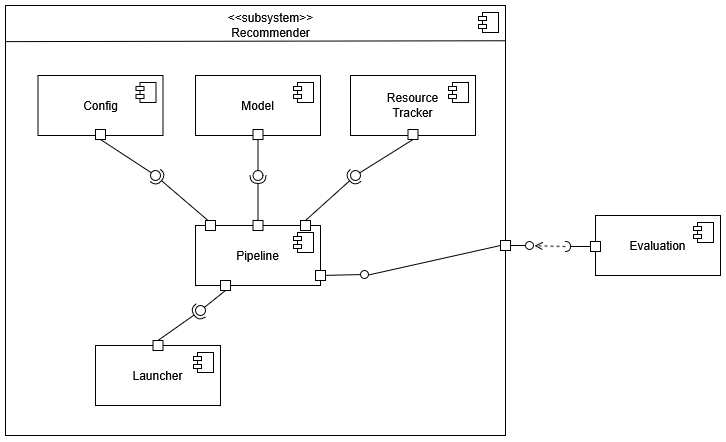
\includegraphics[width=1\textwidth]{img/component.png}
    \caption{Recommender system component diagram}
    \label{fig:component_diagram}
\end{figure}

Here is the deployment setup of the system, including the virtual machine environment and local tools used for development and evaluation:
\begin{figure}[H]
    \centering
    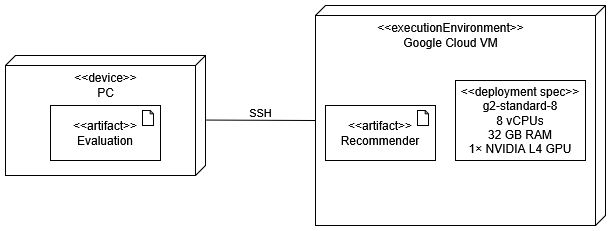
\includegraphics[width=1\textwidth]{img/deployment.png}
    \caption{Deployment diagram}
    \label{fig:deployment_diagram}
\end{figure}


%
%\begin{itemize}
%\item Confidence and p-values
%\item Paired Results - sign test, McNemar's test, paired Student's t-test, Wilcoxon signed rank test
%\item Unpaired Results - Mann-Whitney test
%\item Multiple Tests - ANOVA, Friedman test for ranking
%\item Confidence Intervals - Gaussian distribution, mean, standard dev
%\end{itemize}
%%
%

\clearpage
\section{Evaluation and Results}
This section presents how the recommendation results were evaluated. The goal is to compare the previously mentioned text representation methods, and for comparison there are different metrics to prove which algorithms perform better in which scenarios. When \textbf{Evaluating} a RS there are two main types of evaluation \cite{Zangerle2023}, which are:
\begin{itemize}
\item System-Centric Evaluation
	\begin{itemize}
	\item Algorithmic Aspects - e.g., the predictive accuracy of recommendation algorithms
	\end{itemize}

\item User-Centric Evaluation
	\begin{itemize}
	\item Users' Perspective - how users perceive its quality or the user experience when interacting with the RS
	\end{itemize}
\end{itemize}
%
%
We will focus on System-Centric Evaluation to test the performance of the algorithms and show results based on the metrics listed below.
%
%
\subsection{Metrics for Evaluation}
It is crucial to define how Relevant an item is based on the input item. Since the digital library dataset used in this work does not track user ratings, interactions, or feedback yet, traditional evaluation metrics that rely on relevance from interaction such as Precision, Recall, or NDCG cannot be applied. The dataset provided the full text of books segmented into paragraphs, without any indication of which content users found useful or interesting. So evaluation had to be performed in a user-independent setting based on the internal characteristics of the recommendation results, which meant it was calculated from content similarity between items.
The metrics below describe how the different text representational models were compared, were the Coverage was calculated from a dynamic threshold and the other metrics were computed using the top 10 recommendations per input. This choice was made to focuses on the most similar outputs of each algorithm. 

\begin{itemize}
    \item \textbf{Similarity} – captures how similar each recommended item is to the input item. It is computed using cosine similarity between vectorized representations of the text. The average similarity score across recommendations is used to evaluate how closely the algorithm matches content. Higher similarity will show higher relevance between the compared items in the list of recommended items.

%	\item \textbf{Diversity} – measures how different the recommended items are from each other, ensuring that recommendations cover a broader range of topics or features and are not too similar. There are two common approaches for measuring diversity:
%
%\begin{itemize}
%    \item \textit{Variance of Similarity Scores:} One way to assess diversity is by computing the variance of the pairwise similarity scores among recommended items. A higher variance indicates that the recommendations are spread across a wide range of similarities, while a lower variance indicates that the items are highly similar to each other. This approach focuses on the overall spread of similarity values without directly computing dissimilarity.
%
%    \item \textit{Contrary Effect of Similarity (Dissimilarity):} Alternatively, diversity can be viewed as the inverse of similarity. In this approach, the diversity between two items is calculated as \(1 - \text{cosine similarity}\). The average of all pairwise dissimilarities among recommended items then represents the overall diversity of the recommendation list. This method emphasizes direct measurement of how distinct items are from each other.
%\end{itemize}
%
%Both perspectives aim to ensure a heterogeneous recommendation list, but they differ in their focus: variance-based methods measure spread and consistency, while dissimilarity-based methods explicitly measure distance between items. High diversity values are desirable to avoid recommending nearly identical content and to increase user satisfaction by providing varied and novel options.
%
%Diversity was calculated using similarity-based methods as outlined by Silveira et al. \cite{Silveira2019813}.


	\item \textbf{Diversity} – measures how different the recommended items are from each other, helping to avoid redundant suggestions and offer a wider range of content. It was calculated using two approaches:

\begin{itemize}
    \item \textit{Variance of Similarity Scores:} This method checks how spread out the similarity scores are among recommended items. Higher variance means the items are more varied.
    
    \item \textit{Average Dissimilarity:} This calculates diversity as \(1 - \text{cosine similarity}\), then averages these values to show how distinct the items are from one another.
\end{itemize}

Both methods help ensure that the recommendation list includes a mix of different content types. High diversity improves the chance of covering more topics. These approaches follow the method described Authors in \cite{Silveira2019813}.


	\item \textbf{Confidence} – shows how certain the system is about its recommendations, which was also sampled from top 10 recommendations. It is based on the similarity scores between the input item and the recommended items. Confidence is calculated as the inverse of the standard deviation of these similarity scores:
\[
\text{Confidence} = \frac{1}{1 + \text{std\_dev(similarities)}}
\]
This results in a value between 0 and 1. A higher confidence means that the recommendations are not only strongly related to the input but also consistently similar to each other, indicating that the system is more sure about its recommendations.


	\item \textbf{Coverage} – Catalog Coverage evaluates how effectively a recommendation algorithm utilizes the dataset, measured as the proportion of items in the dataset that are recommended. High item-space coverage indicates that the algorithm explores a wide range of items and is not limited to a small subset. It is calculated as:
\[
\text{Coverage} = \frac{\text{Number of unique recommended items}}{\text{Total number of items in the dataset}} \times 100
\]
To balance the number and relevance (similarity) of recommendations, we used a dynamic thresholding approach so only items scoring above the threshold were recommended. It was set up as a proportion of the maximum similarity per input. Sparse vector models TF-IDF, BoW, LSA and dense BERT embeddings produced lower similarity scores, so a lower threshold (0.5) was used. On the other hand FastText, E5, GloVe returned high similarity scores even for weak matches, requiring stricter thresholds (over 0.9) to avoid overly broad results. We chose these threshold settings to balance recommendation similarity with dataset coverage.

\end{itemize}
In our setup the dataset from GoodReads books contained metadata information to the items such as ratings, number of ratings, number of review and genres. Although this dataset did not include interaction histories (which user selected which book), it allowed for a content-level analysis of recommendation quality through this additional information.

\begin{itemize}
\item \textbf{Novelty} - refers to the fraction of recommended items new to the user, which means they are less known or uncommon items. This metric is based on the assumption that highly rated and popular items are likely to be known to users and therefore not novel. A good measure for novelty might be to look more generally at how well a recommendation system made the user aware of previously unknown items that subsequently turn out to be useful in context.\cite{Avazpour2014245}\\
For our results items were labeled as \textit{novel} if they scored below all three novelty thresholds: below the 25th percentile for rating, number of ratings, and number of reviews. The novelty score was computed as the percentage of top-N recommendations falling into this category.

\item \textbf{Popularity} – captures how frequently recommended items are known or mainstream. Items were labeled as \textit{popular} if they exceeded all three of the following thresholds, derived from the full dataset: above-average rating, above the 75th percentile in number of ratings, and above the 75th percentile in number of reviews. The popularity score of a recommendation set was then calculated as the proportion of top-N recommended items classified as popular.

%\item Usage Prediction - capture the rate of correct recommendations - in a setting where each recommendation can be classified as relevant or non-relevant. Evaluates how well the algorithm predicts whether a user will interact with or use the recommended items, which is based on implicit feedback from the user (clicks, downloads...). Different Metrics can be used to calculate the Usage Prediction, such as Recall, Precision or F-score.

%\item Ranking Measure - evaluates the quality of the ordered list of recommendations by assessing how well the algorithm prioritizes the most relevant item. Relevant recommendations that are ranked higher are scored higher. After the ranking lists are generated by the algorithms, the Ranking Metrics are calculated from their outputs (Precision@K, NDCG@K, MRR).

\end{itemize}

%Also Genre Space Coverage can be mentioned\\

%THRESHOLDS\\
%BERT=0.5\\
%BOW=0.5\\
%FASTTEXT=0.95\\
%GLOVE=099\\
%LSA=0.5\\
%TF-IDF=0.5\\

\begin{figure}[H]
	\centering
	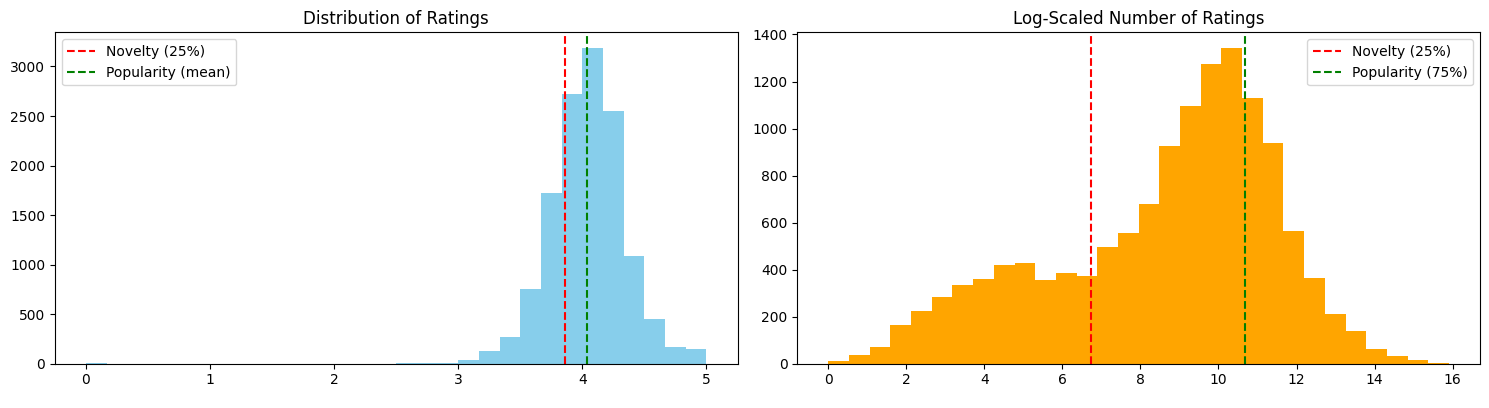
\includegraphics[width=\linewidth,keepaspectratio]{img/ratings_novelty_popularity2.png}
	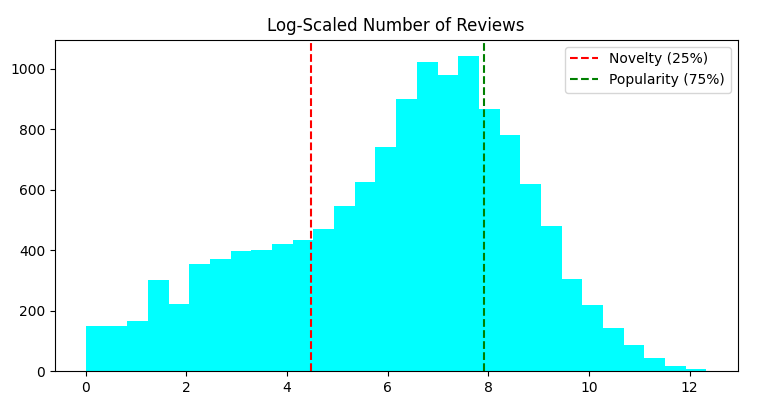
\includegraphics[width=\dimexpr0.5\linewidth\relax,keepaspectratio]{img/ratings_novelty_popularity3.png}
	\caption{Distribution of ratings and reviews in GoodReads dataset}
	\label{fig:ratings_chart}
\end{figure}


\subsection{Results}

The radar charts in Figures~\ref{fig:descriptions_radar} and ~\ref{fig:paragraphs_radar} present a visual comparison of each algorithm’s performance across different evaluation metrics. All values are normalized to a \([0, 1]\) scale to be able to compare them across metrics with different units. The metrics include similarity, confidence, coverage, diversity variance and diversity dissimilarity measures. For the book-description dataset, additional axes for popularity and novelty ratio are also included.
%
%DESCRIPTIONS
%
\begin{figure}[h!]
    \centering
    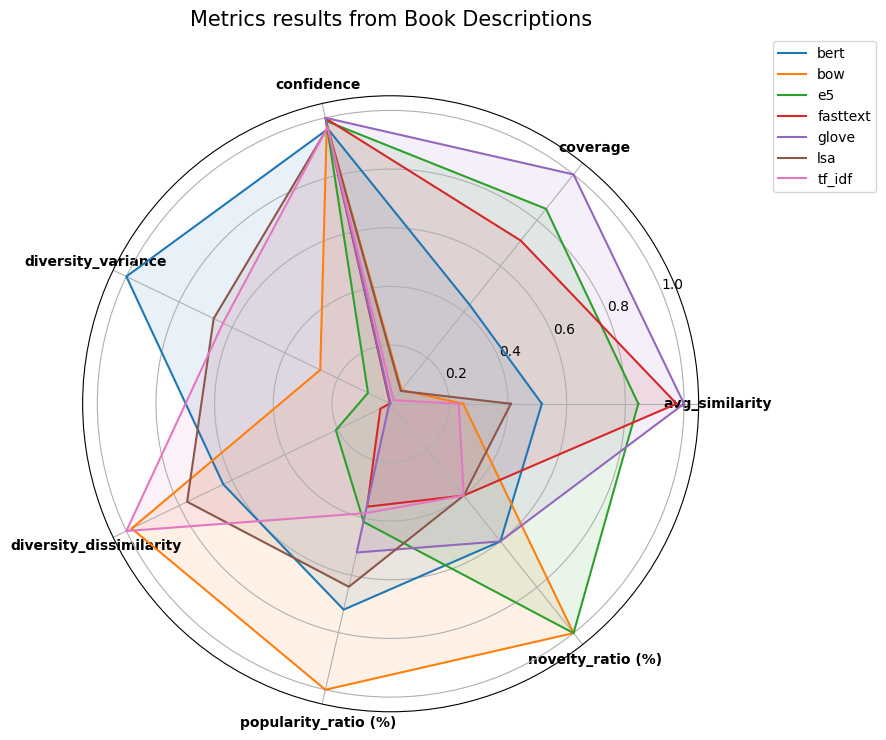
\includegraphics[width=\linewidth,keepaspectratio]{img/descriptions_metrics_radar2.png}
    \caption{Metrics Results of Descriptions Vizualized}
    \label{fig:descriptions_radar}
\end{figure}
%
Figure~\ref{fig:descriptions_radar} shows that GloVe, E5 and Fasttext achieved the highest scores in both coverage and confidence, highlighting their ability to recommend a wide range of items with high semantic consistency. BERT produced the most diverse recommendations in terms of similarity variance, while TF-IDF and BoW scored highest in dissimilarity-based diversity, which means that they returned more varied and less semantically redundant items. Interestingly, BoW also achieved the top scores for popularity and along with E5 they had the highest score for novelty. This may be due to the way BoW works, since it relies on simple keyword overlap. It can recommend very popular items if the input shares common words with them, but it can also suggest less-known books that match on rare or unique words. Because of this, BoW tends to give either very well-known or very unusual results, which helps explain its high scores in both popularity and novelty. E5 embeds entire sentences into dense semantic vectors, capturing deeper contextual meaning, which helps it recommend less typical but still relevant books, which could have resulted in high novelty.

\begin{table}[H]
\centering
\large
\begin{tabular}{|l|c|c|c|c|c|c|c|}
\hline
\textbf{Model} & \textbf{Sim} & \textbf{Cov} & \textbf{Conf} & \textbf{Div (Var.)} & \textbf{Div (Diss.)} & \textbf{Pop (\%)} & \textbf{Nov (\%)} \\
\hline
bert     & 0.513 & 9.29  & 0.96039 & 0.0022251719 & 0.4866 & 18.00 & 3.00 \\
bow      & 0.246 & 1.29  & 0.97755 & 0.0005924999 & 0.7530 & 25.00 & 5.00 \\
e5 		& 0.84 & 18.29 & 0.9883 & 0.0001904935 & 0.1593 & 10.33 & 5.00 \\
fasttext & 0.970 & 15.31 & 0.99765 & 0.0000059949 & 0.0299 & 9.00  & 2.00 \\
glove    & 0.995 & 21.52 & 0.99946 & 0.0000002640 & 0.0045 & 13.00 & 3.00 \\
lsa      & 0.408 & 1.20  & 0.96473 & 0.0014899120 & 0.5917 & 16.00 & 2.00 \\
tf\_idf  & 0.231 & 0.34  & 0.96648 & 0.0014116538 & 0.7684 & 9.56  & 2.00 \\
\hline
\end{tabular}
\caption{Results of Metrics for book descriptions}
\label{tab:metrics_desc}
\end{table}







\begin{table}[H]
\centering
\begin{tabular}{lccccc}

\textbf{Algorithm} & \textbf{CPU Time (s)} & \textbf{RAM (MB)} & \textbf{GPU Mem (MB)}  \\
\hline
BERT     & 27.757 & 1141.38 & 563.78  \\
E5          & 106.777 & 1200.35 & 1732.01 \\
BoW      & 0.275  &  202.89 &  \\
FastText & 11.821 & 1193.43 &\\
GloVe    & 3.210  & 344.33  &\\
LSA      & 2.041  &   424.85  &\\
TF-IDF   & 1.729  &  193.64  &\\

\end{tabular}
\caption{Average resource usage for recommending Book Descriptions}
\label{tab:performance-desc}
\end{table}


\begin{table}[H]
\centering
\begin{tabular}{lccccc}

\textbf{Algorithm} & \textbf{CPU Time (s)}  & \textbf{RAM (MB)} & \textbf{GPU Mem (MB)}\\
\hline
BERT     & 103.399 & 1227.44 & 670.89 \\
E5          & 482.157 & 1313.28 & 1824.2 \\
BoW      & 0.809    & 378.45  & \\
FastText & 44.964   & 2002.80 &  \\
GloVe    & 10.314   & 420.78  & \\
LSA      & 8.179    & 744.64  &  \\
TF-IDF   & 7.230  & 293.49  &  \\

\end{tabular}
\caption{Average resource usage for recommending Book Paragraphs}
\label{tab:performance-paragraph}
\end{table}

The resource usage of each algorithm is shown in Tables~\ref{tab:performance-desc} and~\ref{tab:performance-paragraph}. Deep learning-based models such as BERT, E5 and FastText consumed significantly more CPU time and memory (RAM/GPU), reflecting the cost of their improved similarity results. Traditional models like BoW, TF-IDF, and LSA were computationally lightweight and offered faster execution, which may be better or some systems would prefer it in low-resource environments.


%%%%%%%%%%%%%%%%%%%%%%%%%%%%%%%%%%%%%%%%%%%%%%%%%
% PARAGRAPHS


\begin{figure}[h!]
    \centering
    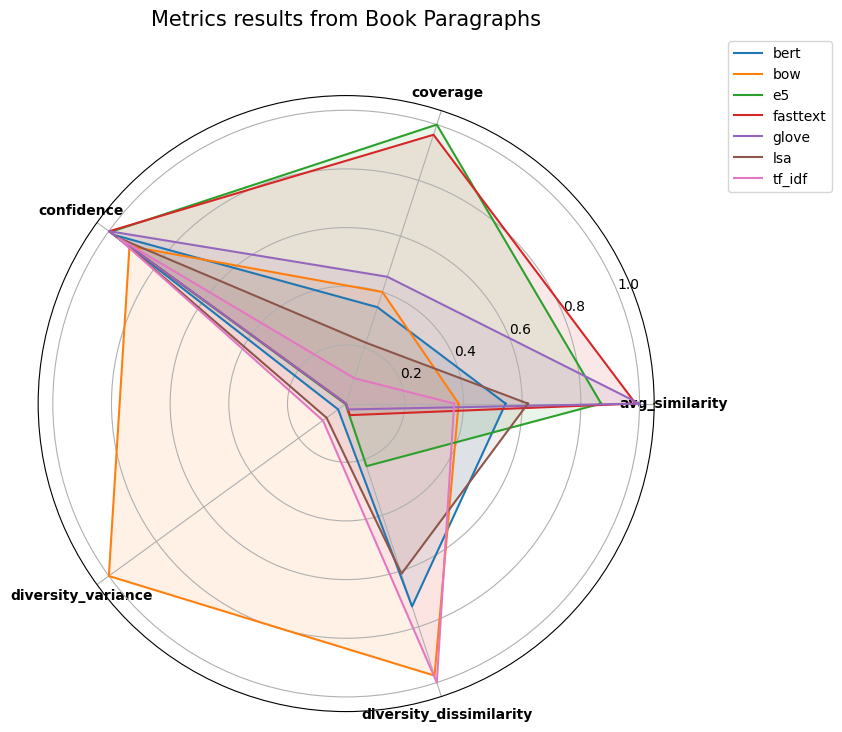
\includegraphics[width=\linewidth,keepaspectratio]{img/paragraphs_metrics_radar2.png}
    \caption{Metrics Results of Paragraphs Vizualized}
    \label{fig:paragraphs_radar}
\end{figure}


Figure~\ref{fig:paragraphs_radar} presents the evaluation results based on paragraph-level recommendations. FastText and GloVe achieved the highest scores in similarity, highlighting their effectiveness in capturing semantic closeness between input and recommended items. E5 and FastText showed the strongest performance in coverage, indicating their ability to recommend a wide range of items across the dataset. Confidence values were highest for FastText, E5 and GloVe, although all models had relatively similar scores, suggesting consistent recommendation strength.


\begin{table}[h!]
\centering
\large
\begin{tabular}{|l|c|c|c|c|c|}
\hline
\textbf{Model} & \textbf{Sim} & \textbf{Cov} & \textbf{Conf} & \textbf{Div (Var.)} & \textbf{Div (Diss.)} \\
\hline
bert     & 0.536 & 0.19 & 0.97654 & 0.0006018049  & 0.463  \\
bow      & 0.378 & 0.22 & 0.91190 & 0.0178139560  & 0.621  \\
e5		& 0.857 & 0.55 & 0.99352 & 0.000048741 & 0.1429 \\
fasttext & 0.973 & 0.53 & 0.99791 & 0.0000068039  & 0.0264 \\
glove    & 0.986 & 0.25 & 0.99877 & 0.0000019924  & 0.0134 \\
lsa      & 0.611 & 0.12 & 0.96231 & 0.0014689289  & 0.3886 \\
tf\_idf  & 0.363 & 0.05 & 0.95945 & 0.0017445470  & 0.6368 \\
\hline
\end{tabular}
\caption{Results of Metrics for book paragraphs}
\label{tab:metrics_para}
\end{table}


In contrast, BoW achieved the highest diversity in variance and TF-IDF achieved it in dissimilarity measures, reflecting their ability to produce a wider range of less semantically redundant results. This comes at the cost of lower similarity, indicating a broader but potentially less targeted recommendation list. BERT provided a balanced performance across most metrics, offering moderately strong similarity, confidence, and diversity.









%%%%%%%%%%%%%%%%%%%%%%%%%%%%%%%%%%%%%%%%%%%%%%%%%%%

\clearpage{}
\section{Conclusion}
% 1 - 2 pages
The field of recommendation algorithms is very popular in academic research. In order to know which type of recommendation method to use our work was set out to evaluate the effectiveness of various content-based recommendation algorithms when applied to digital library datasets.
For comparison two distinct datasets were used in this work, one based on academic book paragraphs and the other from Goodreads containing book descriptions and associated metadata. The project explored the strengths and limitations of seven different text representation methods: \textit{TF-IDF}, \textit{BoW}, \textit{LSA}, \textit{GloVe}, \textit{FastText}, \textit{BERT} and \textbf{E5}, while recommending items based on \textit{Cosine Similarity}.
%
To compare the models in a fair and consistent manner we used a system-centric evaluation approach and we defined metrics such as similarity, diversity, confidence, coverage, novelty, and popularity. These were selected to reflect how similar, consistent, and varied the recommendations were, especially in the absence of user interaction data. Besides those metrics resource consumption was tracked, which showed insights of each algorithm’s performance.
%
To conclude, the results demonstrated that dense embedding models like GloVe, E5 and FastText excelled at finding semantically similar items with strong coverage and confidence, while traditional models like BoW and TF-IDF offered higher diversity and showed some unexpected results in achieving high popularity and novelty scores. BERT and E5 were more resource-intensive, but BERT offered a well-balanced performance across most metrics.
The evaluation pipeline and multi-metric approach ensure that the findings are reproducible and can be adapted for other datasets or domains in the future.



\subsection{Future Work}

While the current system benchmarks several key algorithms in a content-based setting for textual recommendations, there are several directions to further develop and expand the framework.
%
Adding more state-of-the-art models, especially recent advancements in language representation,could make the recommendations even more accurate. The system could also be tested on more types of datasets, like multilingual content, other forms of content or datasets from different domains. There could also be imrpovements made in cleaning and preprocessing the text better as in normalizing or tokenizing differently.
%
Right now, the system only uses content-based methods. In the future, it could also include collaborative or hybrid recommendation approaches, which combine different techniques. However, implementing these approaches would require user interaction data through clicks or ratings to be able to define which items the user selected and better define which recommendations are more relevant.

%Finally, turning the system into an online tool or API would make it easier to use in real applications and allow testing with real users.
%
%Additionally, deploying the system as an interactive tool—via a web interface or API—could allow for real-world usability testing and dynamic evaluation.

%%%%%%%%%%%%%%%%%%%%%%%%%%%%%%%%%%%%%%%%%%%%%%%%%%%
\selectlanguage{slovak}
\clearpage{}
\section*{Resumé}
\addcontentsline{toc}{section}{Resumé}

\subsection*{Úvod}
Odporúčacie systémy sú čoraz dôležitejšie pri filtrovaní veľkého množstva online informácií. Nejde len o úsporu času, ale aj o zlepšenie používateľského zážitku tým, že systém predpovedá, o aký obsah by mohol mať používateľ záujem. Tento projekt sa zameriava na odporúčanie kníh pomocou rôznych algoritmov a ich vyhodnotenie pomocou stanovených metrík.

\subsection*{Pochopenie odporúčacích systémov}

Výskum sa zaoberá porozumením odporúčacích systémov, ich základnými princípmi, typmi a technikami, ktoré sa používajú na generovanie personalizovaných odporúčaní. Predstavili sme rozdiel medzi odporúčacími systémami a vyhľadávačmi. \textbf{Odporúčacie systémy} navrhujú personalizovaný obsah na základe predchádzajúceho správania a preferencií používateľa, zatiaľ čo \textbf{vyhľadávače} vyhľadávajú informácie na základe zadaných kľúčových slov.

Popísali sme hlavné typy odporúčaní vrátane odporúčaní založených na obsahu (content-based), kolaboratívneho filtrovania (collaborative filtering), znalostných grafov (knowledge graphs) a hybridných prístupov. Zamerali sme sa na ich výhody, nevýhody, architektúru a metódy ako napríklad maticovú faktorizácium, využitie sémantických informácií a aj akým spôsobom používajú spätnú väzbu, či už explicitnú (napr. hodnotenia, komentáre od používateľa) alebo implicitnú (napr. počet kliknutí, čas strávený na stránke, história prezerania).

V časti o ťažkostiach odporúčacích systémov sme poukázali na problémy ako studený-štart, riedkosť dát, škálovateľnosť, súkromie a serendipitu. 
Dôležitou súčasťou analýzy bola aj časť o hodnotení týchto systémov, kde sme rozdelili metriky na tie zamerané na presnosť predikcie, predikciu použitia a poradie. Okrem toho sme spomenuli ďalšie metriky ako napríklad dôvera, rôznorodosť, pokrytie, robustnosť a sebaistota odporúčania.

V rámci prehľadu prác v oblasti odporúčacích systémov Beel et al. (2016) ukázali, že viac ako polovica odporúčacích systémov v akademickom prostredí používa odporúčanie založené na obsahu, najmä kvôli absencii spätnej väzby a bohatého textu \cite{Beel2016305}. 

%\textbf{Zangerle et al. (2023)} navrhli rámec FEVR, ktorý systematicky kategorizuje hodnotenie odporúčacích systémov podľa cieľov, metód, dát a metrík a zdôrazňuje potrebu ich spoločného posudzovania~\cite{Zangerle2023}. \textbf{Silveira et al. (2019)} formalizovali šesť hlavných metrík ako úžitok, novosť či serendipitu, rozlíšili ich podľa závislosti od používateľa a navrhli prepojenie online a offline hodnotení~\cite{Silveira2019813}. Na rozdiel od týchto prístupov táto práca využíva content-based filtering pomocou Cosine Similarity nad rôznymi textovými reprezentáciami ako TF-IDF, BoW a BERT, pričom vyhodnocovanie prebieha pomocou metrík nezávislých od používateľa.


\subsection*{Návrh riešenia}

Na základe analýzy bola navrhnutá architektúra systému, ktorý porovnáva viacero algoritmov na odporúčanie kníh. Boli použité dva datasety – prvý obsahuje akademické knihy rozdelené na odseky a druhý obsahuje opisné metadáta z knižnej platformy Goodreads, pokrývajúce rôzne žánre ako fantasy, komédia či romantika. Prístup umožňuje otestovať odporúčania v rôznych kontextoch a textových štruktúrach.

Navrhnutý systém využíva viacero techník na reprezentáciu textu vrátane:
\begin{itemize}
\item TF-IDF – Zohľadňuje dôležitosť slov podľa ich výskytu v dokumente a v celom korpuse; vytvára riedke vektory s váhami slov.
\item Bag of Words (BoW) – Jednoduchá metóda založená na počte výskytov slov bez ohľadu na poradie alebo význam; každé slovo je reprezentované ako samostatná dimenzia.
\item Latent Semantic Analysis (LSA) – Rozširuje TF-IDF pomocou zníženia dimenzionality (SVD), čím odhaľuje skryté vzťahy medzi slovami a dokumentmi.
\item GloVe – Predtrénovaný model vektorov slov založený na frekvencii spoločného výskytu slov v širokom kontexte; vhodný na zachytenie významových vzťahov.
\item FastText – Vylepšuje vektorové reprezentácie slov pomocou znakových n-gramov, čo umožňuje reprezentovať aj neznáme alebo zriedkavé slová.
\item BERT  – Kontextuálny jazykový model využívajúci mechanizmus vlastnej pozornosti (self-attention), ktorý vytvára vektory na úrovni viet s ohľadom na význam slov v danom kontexte.
\item E5 –
\end{itemize}
Tieto metódy pokrývajú spektrum od jednoduchých štatistických modelov až po pokročilé vektorové reprezentácie učené pomocou hlbokých neurónových sietí.

\subsection*{Implementácia}

Systém bol implementovaný v jazyku Python. Použitím knižníc ako pandas, scikit-learn a transformers bolo možné spracovať a implementovať modely na reprezentáciu textu. Kvôli výpočtovo náročním modelom bola použitá virtuálna mašina v Google Cloud s GPU podporou, kde boli jednotlivé algoritmy spustené. Na ukladanie výsledkov odporúčaní, spotreby zdrojov a meraní bol vytvorený jednotný postup.
Základný postup implementácie obsahoval tieto kroky:
\begin{itemize}
\item    Načítanie a predspracovanie dát
\item    Vytvorenie modelov na reprezentáciu textu
\item    Výpočet podobnosti medzi položkami pomocou kosínusovej podobnosti
\item    Filtrovanie a zoradenie výsledkov
\item    Meranie výkonnosti a vyhodnotenie metrických výsledkov
\end{itemize}

\subsection*{Vyhodnotenie a výsledky}

Všetky modely boli porovnané pomocou viacerých metrík:
\begin{itemize}
\item    Podobnosť (Similarity) – miera podobnosti medzi odporúčanými a vstupnými textami
\item    Dôvera (Confidence) – stabilita odporúčaní, založená na podobnostiach medzi vstupom a odporúčanými položkami; počítaná ako inverzná hodnota smerodajnej odchýlky týchto podobností, kde vyššia hodnota znamená konzistentnejšie odporúčania.
\item    Rôznorodosť (Diversity) – rôznorodosť odporúčaných položiek, meraná dvoma spôsobmi: 
(1) ako rozptyl skóre podobnosti medzi odporúčaniami (vyšší rozptyl znamená väčšiu rôznorodosť) 
a (2) ako priemerná nepodobnosť, počítaná ako opak podobnosti.
\item    Pokrytie (Coverage) – podiel odporúčaných položiek z celkového datasetu
\item    Novinka (Novelty) – výskyt menej známych alebo hodnotených položiek
\item    Popularita (Popularity) – podiel často hodnotených alebo populárnych položiek
\end{itemize}



Na základe metrík a analýzy výkonu boli pozorované nasledovné výsledky:
\begin{itemize}
\item    FastText a GloVe dosiahli vysokú podobnosť, pokrytie a dôveru.
\item    BERT priniesol najvyváženejšie výsledky, ale s vyššou náročnosťou na výpočtové zdroje.
\item    Tradičné modely ako BoW a TF-IDF ponúkli vysokú diverzitu a zároveň zaujímavý pomer populárnych aj nových odporúčaní.
\end{itemize}
Okrem kvalitatívneho hodnotenia boli zaznamenané aj časy spracovania, spotreba RAM a GPU pamäte. Tieto informácie umožňujú lepšie rozhodovanie o výbere modelov v rôznych prostrediach.

\subsection*{Záver}
Práca preukázala, že výber reprezentácie textu výrazne ovplyvňuje výsledky odporúčania. Moderné metódy ako FastText či GloVe poskytujú vysoko podobné odporúčania, zatiaľ čo jednoduchšie metódy ako BoW môžu priniesť väčšiu rôznorodosť a popularitu. Navrhnutý systém je modulárny a rozšíriteľný, čo umožňuje jeho ďalší vývoj v akademickom aj praktickom prostredí.

\subsubsection*{Možnosti ďalšieho rozšírenia}
Budúci vývoj systému by mohol zahŕňať:
zapojenie novších modelov na spracovanie prirodzeného jazyka (napr. veľké jazykové modely),
testovanie na viac typoch datasetov (viacjazyčné texty),
vylepšenie predspracovania textu a čistenia údajov,
začlenenie kolaboratívneho alebo hybridného odporúčania, ktoré si však vyžaduje dáta so spätnou väzbou od používateľov.
V konečnom dôsledku je systém vhodný na ďalšie testovanie, rozšírenie do webovej aplikácie alebo reálne použitie v digitálnych knižniciach.


%%%%%%%%%%%%%%%%%%%%%%%%%%%%%%%%%%%%%%%%%%%%%%%%%%%
\selectlanguage{english}
\clearpage 
\section*{References} % No numbering
\addcontentsline{toc}{section}{References} % Add to TOC
\renewcommand{\refname}{}

\normalsize 
\bibliographystyle{unsrt} 
\bibliography{literature} 
\nocite{*}

%%%%%%%%%%%%%%%%%%%%%%%%%%%%%%%%%%%%%%%%

\clearpage
\appendix

\renewcommand{\thepage}{A-\arabic{page}}
\setcounter{page}{1}
\subsection*{Appendix A: Plan of Work} % No numbering
\addcontentsline{toc}{section}{Appendix A: Plan of Work} % Add to TOC
\renewcommand{\refname}{}

Here is an overview of the work throughout the year 2024/2025 for the Bachelor's Thesis.

\begin{longtable}{|p{2.5cm}|p{12cm}|}
\hline
\textbf{Week} & \textbf{Planned Work Description} \\
\hline
\multicolumn{2}{|c|}{\textbf{Semester 1 – Research and Proposal}} \\
\hline
Weeks 1--2 & The topic will be selected and initial research on recommender systems will be conducted. Relevant literature on RS types, filtering techniques, and evaluation strategies will be reviewed. \\
\hline
Weeks 3--4 & Detailed research and analysis of different types of recommender systems will be carried out. \\
\hline
Weeks 5--6 & The recommender systems will be analyzed. The project scope will be defined, with a focus on the appropriate recommender method for digital library use cases. \\
\hline
Weeks 7--8 & The evaluation methodology will be designed, including the selection of different metrics. \\
\hline
Weeks 9--10 & Datasets will be collected: academic paragraphs and additionally other public datasets. \\
\hline
Weeks 11--12 & A proposal will be written, outlining the implementation strategy for the book recommendation system and the evaluation plan. \\
\hline

\multicolumn{2}{|c|}{\textbf{Semester 2 – Implementation and Evaluation}} \\
\hline
Weeks 1--2 & A JSON parser will be implemented, and the data will be structured using Python. Experiments with various text representation models will be initiated. \\
\hline
Weeks 3--4 & A recommendation pipeline based on cosine similarity and resource tracking will be developed. A Virtual Machine environment will be set up for conducting experiments. \\
\hline
Weeks 5--6 & Offline experiments will be run on the datasets using all selected models, and outputs and similarity scores will be collected. \\
\hline
Weeks 7--8 & Evaluation metrics will be computed. System performance will be logged (CPU, RAM, GPU usage). Visual outputs such as diagrams, radar plots, and deployment overviews will be finalized. \\
\hline
Weeks 9--10 & The chapters on implementation, evaluation, and conclusion will be written, focusing on the interpretation of results. \\
\hline
Weeks 11--12 & All chapters will be reviewed and finalized. Appendices and source documentation will be completed to finalize the thesis project. \\
\hline
\end{longtable}

%=====================================================%

\clearpage
\renewcommand{\thepage}{B-\arabic{page}}
\setcounter{page}{1}
\subsection*{Appendix B: Technical Documentation} % No numbering
\addcontentsline{toc}{section}{Appendix B: Technical Documentation} 
\renewcommand{\refname}{}
The technical documentation was written in markdown format for the github repository and is attached as an appendix.\\
Here is the link to find the repository for the documentation, implementation and results: \\
\href{https://github.com/Akos360/Evaluating\_Recommender\_Systems\_Implementation.git}{github.com/Akos360/Evaluating\_Recommender\_Systems\_Implementation}
\clearpage
\renewcommand{\thepage}{C-\arabic{page}}
\setcounter{page}{1}
\subsection*{Appendix C: 2025 IIT.SRC Conference} 
\addcontentsline{toc}{section}{Appendix C: 2025 IIT.SRC Conference} 
\renewcommand{\refname}{}
Article created for IIT.SRC 2025: \textbf{Evaluating Recommender Systems for Digital Library Datasets}
\includepdf[pages=-]{opraveny_iitsrc.pdf}


\clearpage
\renewcommand{\thepage}{D-\arabic{page}}
\setcounter{page}{1}
\subsection*{Appendix D: DEMOcon 2025} 
\addcontentsline{toc}{section}{Appendix D: DEMOcon 2025} 
\renewcommand{\refname}{}
Article created for DEMOcon 2025: \textbf{Evaluating Recommender Systems for Digital Library Datasets}
\includepdf[pages=-]{DemoCon.pdf}

\clearpage
\renewcommand{\thepage}{E-\arabic{page}}
\setcounter{page}{1}
\subsection*{Appendix E: Digital Attachments} 
\addcontentsline{toc}{section}{Appendix E: Digital Attachments} 
\renewcommand{\refname}{}
\textnormal{
Here is the link to find the repository for the documentation, implementation and results: \\
\href{https://github.com/Akos360/Evaluating\_Recommender\_Systems\_Implementation.git}{github.com/Akos360/Evaluating\_Recommender\_Systems\_Implementation}}


\end{document}
